\documentclass[12pt]{article}

% --- Essential Packages ---
\usepackage[margin=1in]{geometry}
\usepackage{setspace}
\onehalfspacing

\usepackage{amsmath, amssymb, amsfonts, mathtools}
\usepackage{graphicx}
\usepackage{booktabs}
\usepackage{array}
\usepackage{tabularx}
\usepackage{float}
\usepackage[labelfont=bf, font=small, skip=6pt]{caption}
\usepackage{subcaption}
\usepackage{microtype}
\usepackage{xcolor}
\usepackage{natbib}

% --- Hyperref Setup ---
\usepackage[
  colorlinks=true,
  linkcolor=blue!70!black,
  citecolor=blue!70!black,
  urlcolor=blue!70!black,
  pdftitle={Identifying Personal Network Types: Structural Topologies, Empirical Decision Rules, and Longitudinal Transitions},
  pdfauthor={Omar Lizardo, Brandon Sepulvado, Cheng Wang, David Hachen}
]{hyperref}
\usepackage[capitalize,noabbrev]{cleveref}

% --- Custom Math Operators & Styling ---
\DeclareMathOperator*{\argmin}{arg\,min}
\newcommand{\xbar}{\bar{x}}

\title{\textbf{Identifying Personal Network Types: Structural Topologies, Empirical Decision Rules, and Longitudinal Transitions in a Collegiate Setting}}

\author{
  David Hachen\thanks{Department of Sociology, University of Notre Dame.} \quad
  Omar Lizardo\thanks{Department of Sociology, University of California, Los Angeles.} \quad
  Brandon Sepulvado\thanks{NORC.} \quad
  Cheng Wang\thanks{Department of Sociology, Wayne State University.} 
}

\date{September 2026}

\begin{document}

\maketitle

\begin{abstract}
\noindent Building on foundational work by \citet{bidart2018personal} and \citet{vacca2020structure}, we investigate whether ego networks can be classified into discrete types based on their structural signatures using eight survey waves from the NetHealth Study ($N = 701$). Using unsupervised $k$-means clustering on ego-network topological metrics, we recover four configurations corresponding to types discussed in previous work: ``Pearl Collar Networks'' (large, modular, high-diameter), ``Segmented Networks'' (moderately sized, decentralized), ``Centered Star Networks'' (highly centralized around key intermediaries), and ``Regular Dense Networks'' (small, cohesive, tightly knit). With this classification in hand, we extend prior scholarship in three major directions. First, we use empirical classification trees to predict individual membership in each ego-network type with 92.9\% accuracy, establishing explicit, data-driven cutoffs for values of each structural signature to determine membership in each type. Second, we use longitudinal Markov models across 1,900 transitions to examine the dynamic evolution of individuals across types, revealing high persistence in regular dense network structures (70.8\%) alongside substantial structural mobility across the other types. Third, we use multilevel multinomial models with crossed random effects for residence halls ($J = 29$) and academic majors ($J = 43$) to show that institutional opportunity structures, gender identity, international status, and individual personality dispositions jointly sort individuals into distinct personal network regimes.

\vspace{1ex}
\noindent \textbf{Keywords:} Personal networks, egocentric network analysis, structural typologies, classification trees, Markov models, multilevel multinomial logit, social support.
\end{abstract}

\clearpage

\section{Introduction}

The study of ego networks occupies a central position in network analysis, linking macro-level institutional configurations to micro-level interpersonal interactions \citep{smith2020introduction, perry2018egocentric}. Early efforts to categorize personal networks were predominantly attribute-based, classifying networks according to role relationships, such as the balance between kin and non-kin, or the specific forms of social support exchanged across ties \citep{antonucci2013convoy, offer2018does}. While informative about relational content, these compositional approaches often overlooked the overarching topological geometry of the ego network---the formal patterns of connectivity, cohesion, and segmentation that govern resource flows, social capital, and information diffusion among alters and between ego and alters. When structural signatures were used, they were often limited to basic network statistics such as size and clustering \citep{burt1992structural, marsden1987core}. More recent work has gone beyond this approach, using a richer set of structural signatures, built from alter-to-alter patterns of connectivity, to develop data-driven typologies that classify ego-networks into theoretically meaningful types \citep{bidart2018personal, giannella2016inductive, vacca2020structure}.

Our analysis extends previous scholarship in six substantive directions. We begin by mapping the correlation matrix of egocentric graph metrics, showing how subgroup modularity and dyadic density systematically trade off as personal networks expand in volume. To ground these structural signatures in concrete social configurations, we draw on Vacca's \citeyearpar{vacca2020structure} emphasis on medoid representations to identify empirical archetype exemplars and visualize their relational structures using force-directed network graphs. Moving beyond manual heuristics and algorithmic clustering assignments, we then train an empirical classification decision tree that predicts typology membership with 92.9\% accuracy and establishes explicit topological cutoffs. Overcoming the static constraints of cross-sectional surveys, we evaluate semester-to-semester Markov state transitions across 1,900 longitudinal intervals to measure the empirical stability and structural mobility of personal network forms over time. Next, we connect these relational configurations to institutional opportunity structures and individual dispositions by estimating multilevel categorical logit models with crossed random effects for freshman residence halls ($J = 29$) and academic majors ($J = 43$) alongside validated Big Five personality dimensions. Finally, we bridge the longstanding divide between structural and compositional network traditions by examining functional social support provisions, revealing how topological structure governs relational multiplexity and emotional bandwidth.

\section{Recent Developments in Personal Network Typologies}

The ambition to classify personal networks into discrete structural types represents an enduring program within sociocentric and egocentric analysis. Rather than treating personal networks as undifferentiated aggregations of ties, typology research seeks to uncover recurrent configurations of interpersonal relations that reflect fundamental principles of social organization \citep{fischer1982dwell, mccarty2002structure, perry2018egocentric}. Over the past two decades, this literature has progressed across four interrelated currents: (1) the transition from attribute-based compositional profiles to purely topological graph structures; (2) the debate between deductive theoretical archetypes and inductive algorithmic clustering; (3) alternative frameworks centered on structural cohesion, fragmentation, and hierarchical deconstruction; and (4) the emerging connection between individual psychological dispositions and network ego network structural signatures.

\subsection{The Compositional vs.\ Structural Divide in Network Typologizing}

Early typological research predominantly focused on network composition---the demographic attributes, role categories, and institutional contexts characterizing an individual's contacts \citep{antonucci2013convoy, offer2018does}. In a recent influential contribution in this tradition, \citet{giannella2016inductive} used Random Forests on detailed survey data from Northern California ($N = 1{,}050$) to derive an inductive typology of egocentric networks. Combining over 40 survey descriptors into seven core dimensions (such as non-kin interaction, kin proximity, kin support, church, and work involvement), they reliably placed respondents into seven distinct profiles: ``career-and-friends'' (24\%), ``family-and-community'' (20\%), ``family-only'' (16\%), ``untethered'' (8\%), ``energetic'' (7\%), ``withdrawn'' (6\%), and ``home-and-church'' (5\%).

Subsequent scholarship has extended this compositional paradigm to large national panels and vulnerable populations. \citet{laier2022inductive} applied the Random Forest framework to the German Socio-Economic Panel (SOEP, $N = 8{,}341$), identifying fine-grained compositional types based on core discussion networks to show how relational repertoires evolve across the life course. \citet{pelle2021clustering} developed a distance-based clustering methodology for mixed-type survey data from the Italian National Statistical Institute ($N = 4{,}495$), grouping elderly individuals living alone into distinct vulnerability profiles based on contact frequency, support type, and kin availability. Extending this logic to romantic dyads, \citet{kennedy2023typologies} introduced the concept of ``duocentric networks'' among low-income newlyweds ($N = 207$), clustering couples by spousal network overlap and the balance between family and friend ties to reveal how shared relational ecologies shape marital support.

Yet, as \citet{mccarty2002structure} argued in an early intervention, compositional summaries treat the personal network as an unordered collection of alters, completely obscuring the structural patterns connecting alters to one another. McCarty showed that eliciting large personal networks (60 alters and 1,770 evaluated pairs) reveals substantial structural heterogeneity in network density, component counts, and cohesive subgroups that cannot be predicted from ego--alter attributes. Because the topological geometry of alter--alter ties governs resource flows, social capital, normative constraints, and behavioral autonomy \citep{burt1992structural, coleman1988social, granovetter1973strength}, classifying personal networks strictly by their structural topology provides a more direct window into the relational mechanisms that organize social life.

\subsection{Deductive Theoretical Archetypes vs.\ Inductive Clustering}

The pursuit of purely structural typologies reached a turning point with \citet{bidart2018personal}, who analyzed longitudinal qualitative and network data from young adults in France ($N = 87$). Rejecting compositional descriptors, \citeauthor{bidart2018personal} formulated six theoretical archetypes defined solely by alter--alter graph metrics: ``Regular Dense'' (small, single-clique enclosures), ``Centered Dense'' (dense cores surrounded by peripheral nodes), ``Centered Star'' (radial networks dominated by central broker alters), ``Segmented'' (decentralized, disconnected components), ``Pearl Collar'' (multiple distinct cliques linked sequentially in a ring or pathway), and ``Dispersed'' (fragmented, sparse collections of isolates). To assign networks to these archetypes, they proposed a deductive classification tree based on heuristic cutoff values for alter--alter density, Freeman betweenness centralization ($> 0.20$), diameter, and component shares. While theoretically compelling, \citeauthor{bidart2018personal}'s framework relied on subjective cutoffs derived from a modest sample, raising questions about whether their archetypes reflected universal structural forms or idiosyncratic artifacts of their analytical rules.

To evaluate this question systematically, \citet{vacca2020structure} conducted a comparative investigation across six diverse cross-sectional datasets ($N = 1{,}460$), encompassing immigrants in Southern Europe, disaster survivors in Florida and Ecuador, residents of segregated neighborhoods, and a representative Bay Area sample. Vacca developed an inductive community-detection method using Girvan--Newman modularity partitioning to summarize personal network structure through three properties: the number of cohesive subgroups ($\ge 3$ nodes), the number of isolated dyads/singletons, and partition modularity. By applying $k$-medoids clustering to these metrics, Vacca showed that personal network structures naturally coalesce into distinct inductive groups. Crucially, Vacca revealed substantial discordance and cross-classification between \citeauthor{bidart2018personal}'s deductive assignments and inductive cluster solutions. Inductive clustering demonstrated that empirical networks rarely conform cleanly to rigid theoretical boundaries, underscoring the need for data-driven classification methods that capture authentic structural variation.

\subsection{Cohesion, Fragmentation, and Hierarchical Deconstruction}

Parallel to the Bidart--Vacca contributions, a complementary line of scholarship has examined the fundamental dimensions underlying structural variation. In representative urban surveys in Spain ($N = 403$), \citet{mayajariego2015living} used exploratory factor analysis on density, centralization, clique counts, and components, showing that personal network variability is organized along two primary axes: structural cohesion and fragmentation. Building on this foundation, \citet{mayajariego2021building} developed a structural classification based on centralization, the number of cliques, and component counts, identifying four empirical ego-network types: ``dense,'' ``intermediate,'' ``clustered,'' and ``fragmented.`` These studies showed that individual differences in interpersonal environments are primarily structured by the tension between cohesive solidarity and subgroup fragmentation.

Moving beyond static graph metrics, \citet{mayajariego2023use} introduced a ``hierarchical deconstruction procedure'' that evaluates network topology by iteratively eliminating nodes with the highest betweenness centrality. Analyzing longitudinal networks of 69 university students, they found that dense, highly cohesive networks exhibit prolonged resistance to fragmentation, whereas networks organized around brokerage rapidly deconstruct into disjoint components. This iterative deconstruction showed that personal networks possess hierarchical, nested subgroup structures that determine their resilience to disruption.

Most recently, \citet{gonzalezcasado2024towards} addressed the critique that previous typology studies relied on ad-hoc, arbitrarily selected graph metrics. Analyzing four extensive datasets across Spain and Ecuador, they applied systematic dimensionality reduction (PCA and UMAP) across a comprehensive battery of over 14 topological metrics (including transitivity, path length, degree dispersion, modularity, and centralization). Their findings showed that the structural space of personal networks is overwhelmingly governed by two universal axes: (1) global cohesion (the fundamental mathematical tradeoff between network size and density) and (2) internal structural differentiation (the balance between modular community segregation and centralized brokerage).

\subsection{Psychological Dispositions versus Contextual Effects}

Finally, an emerging line of work connects structural network typologies to individual agency and psychological dispositions. \citet{mayajariego2020personal} examined the relationships among Big Five personality traits, psychological sense of community, and personal network structure in 100 adults. Using modified triadic censuses and global graph metrics, they found that Emotional Stability was positively correlated with network density and closed triads, while psychological sense of community was strongly associated with cohesive triadic embedding. However, their sample was cross-sectional and exploratory, leading the authors to emphasize that future scholarship must incorporate validated personality inventories into multivariate typology models.

\subsection{Extant Gaps in the Current Literature}

Despite these significant methodological advances, the existing literature on personal network typologies exhibits four critical gaps: First, virtually all prior structural typology studies \citep{gonzalezcasado2024towards, mayajariego2021building, mccarty2002structure, vacca2020structure} rely strictly on single cross-sectional snapshots. Even longitudinal studies \citep{bidart2018personal, mayajariego2023use} lacked the sample scale or analytical framework to model state transitions across structural types. Accordingly, whether personal network types represent permanent individual traits or dynamic developmental regimes through which individuals transition over time remains an open empirical question. Second, methodologically, researchers remain trapped between \citeauthor{bidart2018personal}'s transparent but arbitrary manual heuristics and \citeauthor{vacca2020structure}'s or \citeauthor{gonzalezcasado2024towards}'s inductive clustering algorithms, which assign cluster memberships within a given sample as an algorithmic ``black box'' without providing explicit, portable decision rules that other scholars can readily apply. Third, prior studies have largely treated personal networks as self-contained interpersonal systems or compared aggregate national populations without modeling the immediate organizational foci \citep{feld1981focused} in which relationships are forged. How much of the variation in personal network structure is driven by meso-level institutional sorting (such as residential dormitories or academic curricula) versus individual tendencies to select particular types of alters is still not known. Finally, typological research has remained almost entirely structural and descriptive, focusing on defining and comparing topological forms without examining how different network structures systematically shape substantive social support, relational multiplexity, and affective tie closeness.

The present study addresses each of these four limitations by leveraging the NetHealth Study's longitudinal design, institutional setting, and relational depth. First, to overcome the cross-sectional constraint, we analyze eight waves of survey data tracking an undergraduate cohort across their first three collegiate years. This multi-wave design allows us to examine both cumulative relational capital accumulated across college ($N = 701$) and semester-to-semester Markov state transitions ($N = 1{,}900$ intervals), directly evaluating the empirical persistence versus structural mobility of personal network regimes over time. Second, to resolve the dilemma between arbitrary heuristics and uninterpretable algorithmic clustering, we train an empirical classification decision tree that reproduces unsupervised cluster assignments with 92.9\% accuracy. This model yields explicit, data-driven cutoffs---identifying alter--alter density as the primary structural boundary in dense collegiate environments---offering transparent and portable decision criteria that can be applied in comparative research. Third, to address the contextual void, we embed personal networks within their meso-level organizational settings \citep{feld1981focused}, estimating multilevel categorical logit models with crossed random effects for freshman residence halls ($J = 29$) and academic majors ($J = 43$). By partitioning institutional sorting alongside validated Big Five personality dimensions, we quantitatively assess how organizational opportunity structures and individual dispositions jointly shape personal network structure. Finally, to connect abstract topology to substantive social capital, we evaluate alter-level functional support provision across four key domains (social companionship, informational advice, emotional comfort, and financial assistance) alongside composite measures of support multiplexity, relational closeness, and interpersonal trust ($N = 580$).

\section{Data and Analytical Sample}

The empirical analysis draws on the NetHealth Study \citep{liu2018network, sepulvado2020predicting, wang2020neither}, a longitudinal investigation that followed an incoming cohort of undergraduate students over four years of college at the University of Notre Dame. Network surveys were administered online via Qualtrics at the beginning and conclusion of each semester across eight distinct waves between Fall 2015 and Spring 2018. The survey used an open-ended name-generator approach, asking respondents to name up to 20 individuals with whom they communicated or interacted. Beginning in Wave 3, respondents could additionally retain up to five alters from the preceding wave, allowing for up to twenty-five named alters per wave. Name interpreters recorded demographic and relational traits for each alter, and respondents completed alter--alter matrices indicating which of their nominated alters knew one another.

Across all eight survey waves, participants generated 35,912 ego--alter nominations and 174,748 alter--alter evaluations. To capture the full scope of interpersonal connectivity realized during college, we constructed cumulative undirected ego networks by combining all unique alters and realized alter--alter ties reported by each participant across the observation period. Following established methodological criteria for egocentric graph analysis, we restricted the analytic sample to participants who named at least three alters and who reported at least one realized tie between alters. This filtering eliminated isolated dyads and participants with degenerate alter graphs, yielding a final analytic sample of $N = 701$ participants with complete network and demographic data.

\begin{table}[htbp]
\centering
\caption{Descriptive Statistics of Personal Network Structural Metrics by Typology ($N = 701$)}
\label{tab:structural_metrics}
\resizebox{\linewidth}{!}{%
\begin{tabular}{lccccc}
\toprule
\textbf{Structural Metric} & \textbf{Full Sample} & \textbf{Pearl Collar} & \textbf{Segmented} & \textbf{Centered Star} & \textbf{Regular Dense} \\
 & \textbf{($N = 701$)} & \textbf{($n = 176$)} & \textbf{($n = 261$)} & \textbf{($n = 143$)} & \textbf{($n = 121$)} \\
\midrule
Network Size                 & 28.8 (16.0)  & 47.9 (14.0)  & 27.4 (10.1)  & 21.6 (8.2)   & 12.6 (6.5)  \\
Community Modularity         & 0.31 (0.17)  & 0.46 (0.11)  & 0.33 (0.13)  & 0.31 (0.11)  & 0.07 (0.07) \\
Network Diameter             & 3.2 (1.3)    & 4.5 (1.2)    & 2.7 (0.8)    & 3.4 (0.9)    & 1.9 (0.6)   \\
Betweenness Centralization   & 0.19 (0.15)  & 0.22 (0.11)  & 0.11 (0.07)  & 0.40 (0.12)  & 0.06 (0.07) \\
Alter--Alter Density         & 0.38 (0.21)  & 0.21 (0.06)  & 0.33 (0.11)  & 0.37 (0.10)  & 0.77 (0.15) \\
Transitivity (Clustering)    & 0.73 (0.15)  & 0.64 (0.10)  & 0.74 (0.14)  & 0.68 (0.13)  & 0.88 (0.09) \\
Largest Component Share (\%) & 87.0\% (18.7)& 85.6\% (17.5)& 77.3\% (22.3)& 97.8\% (5.1) & 97.2\% (6.3)\\
\bottomrule
\end{tabular}%
}
\vspace{1ex}
\parbox{\linewidth}{\footnotesize \textit{Note:} Standard deviations are reported in parentheses. Size represents the count of unique alters. Centralization refers to Freeman alter--alter betweenness centralization. Modularity is computed via the Louvain community detection algorithm on alter--alter ties. Largest component share indicates the proportion of alters belonging to the largest connected component.}
\end{table}


\begin{figure}[htbp]
\centering
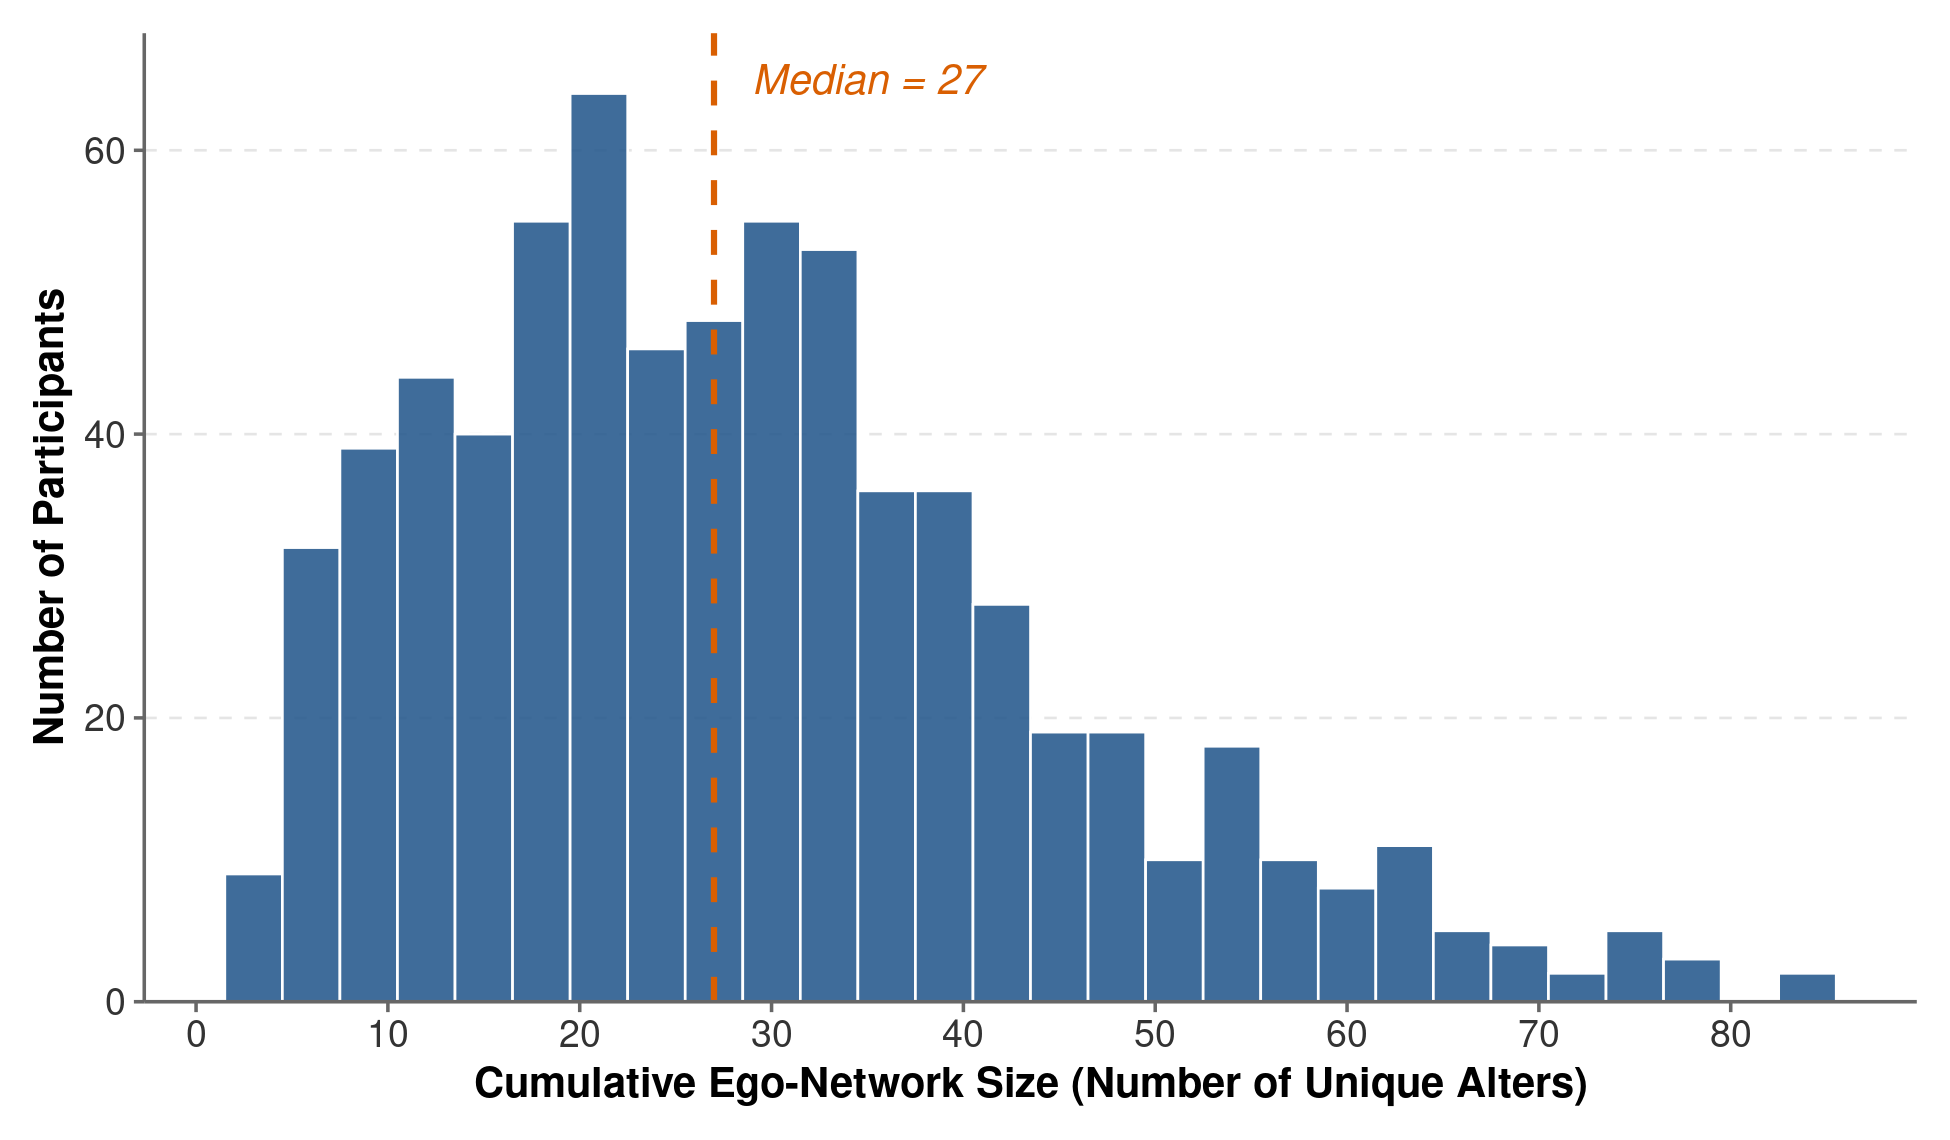
\includegraphics[width=0.85\linewidth]{Plots/fig1_size_distribution.png}
\caption{Cumulative Ego-Network Size Distribution Across NetHealth Participants}
\label{fig:size_distribution}
\vspace{1ex}
\parbox{\linewidth}{\footnotesize \textit{Note:} Distribution of unique alters nominated across Waves 1 through 8 for analytic-sample participants ($N = 701$). The dashed vertical line indicates the sample median of 26 alters; the solid curve represents kernel density smoothing.}
\end{figure}

\Cref{tab:structural_metrics} reports descriptive statistics for the personal network structural metrics across the full analytic sample and within each extracted typology. \Cref{fig:size_distribution} shows the distribution of cumulative ego-network size across the study cohort. The empirical spread underscores that static single-wave snapshots substantially underestimate the total volume of social ties maintained by young adults in residential campus environments. The right tail extends beyond 80 cumulative contacts, with an average of 28.8 alters ($\text{SD} = 16.0$) and a median of 26 alters, highlighting the capacity of highly engaged individuals to sustain extensive interpersonal environments over time.

\section{Structural Network Typologies}

To classify personal networks into structural types without imposing \textit{ex ante} categories, we standardized five core graph metrics ($z$-scores): network size ($n_i$), dyadic density ($d_i$), Louvain community modularity ($Q_i$), graph diameter of the largest connected component ($D_i$), and Freeman alter--alter betweenness centralization ($C_{B, i}$). Formally, each ego network $i$ is represented by a standardized feature vector $\mathbf{z}_i \in \mathbb{R}^5$:
\begin{equation}
\mathbf{z}_i = \left( \frac{n_i - \bar{n}}{\text{SD}(n)}, \; \frac{d_i - \bar{d}}{\text{SD}(d)}, \; \frac{Q_i - \bar{Q}}{\text{SD}(Q)}, \; \frac{D_i - \bar{D}}{\text{SD}(D)}, \; \frac{C_{B, i} - \bar{C}_B}{\text{SD}(C_B)} \right)^\top
\end{equation}

\begin{figure}[htbp]
\centering
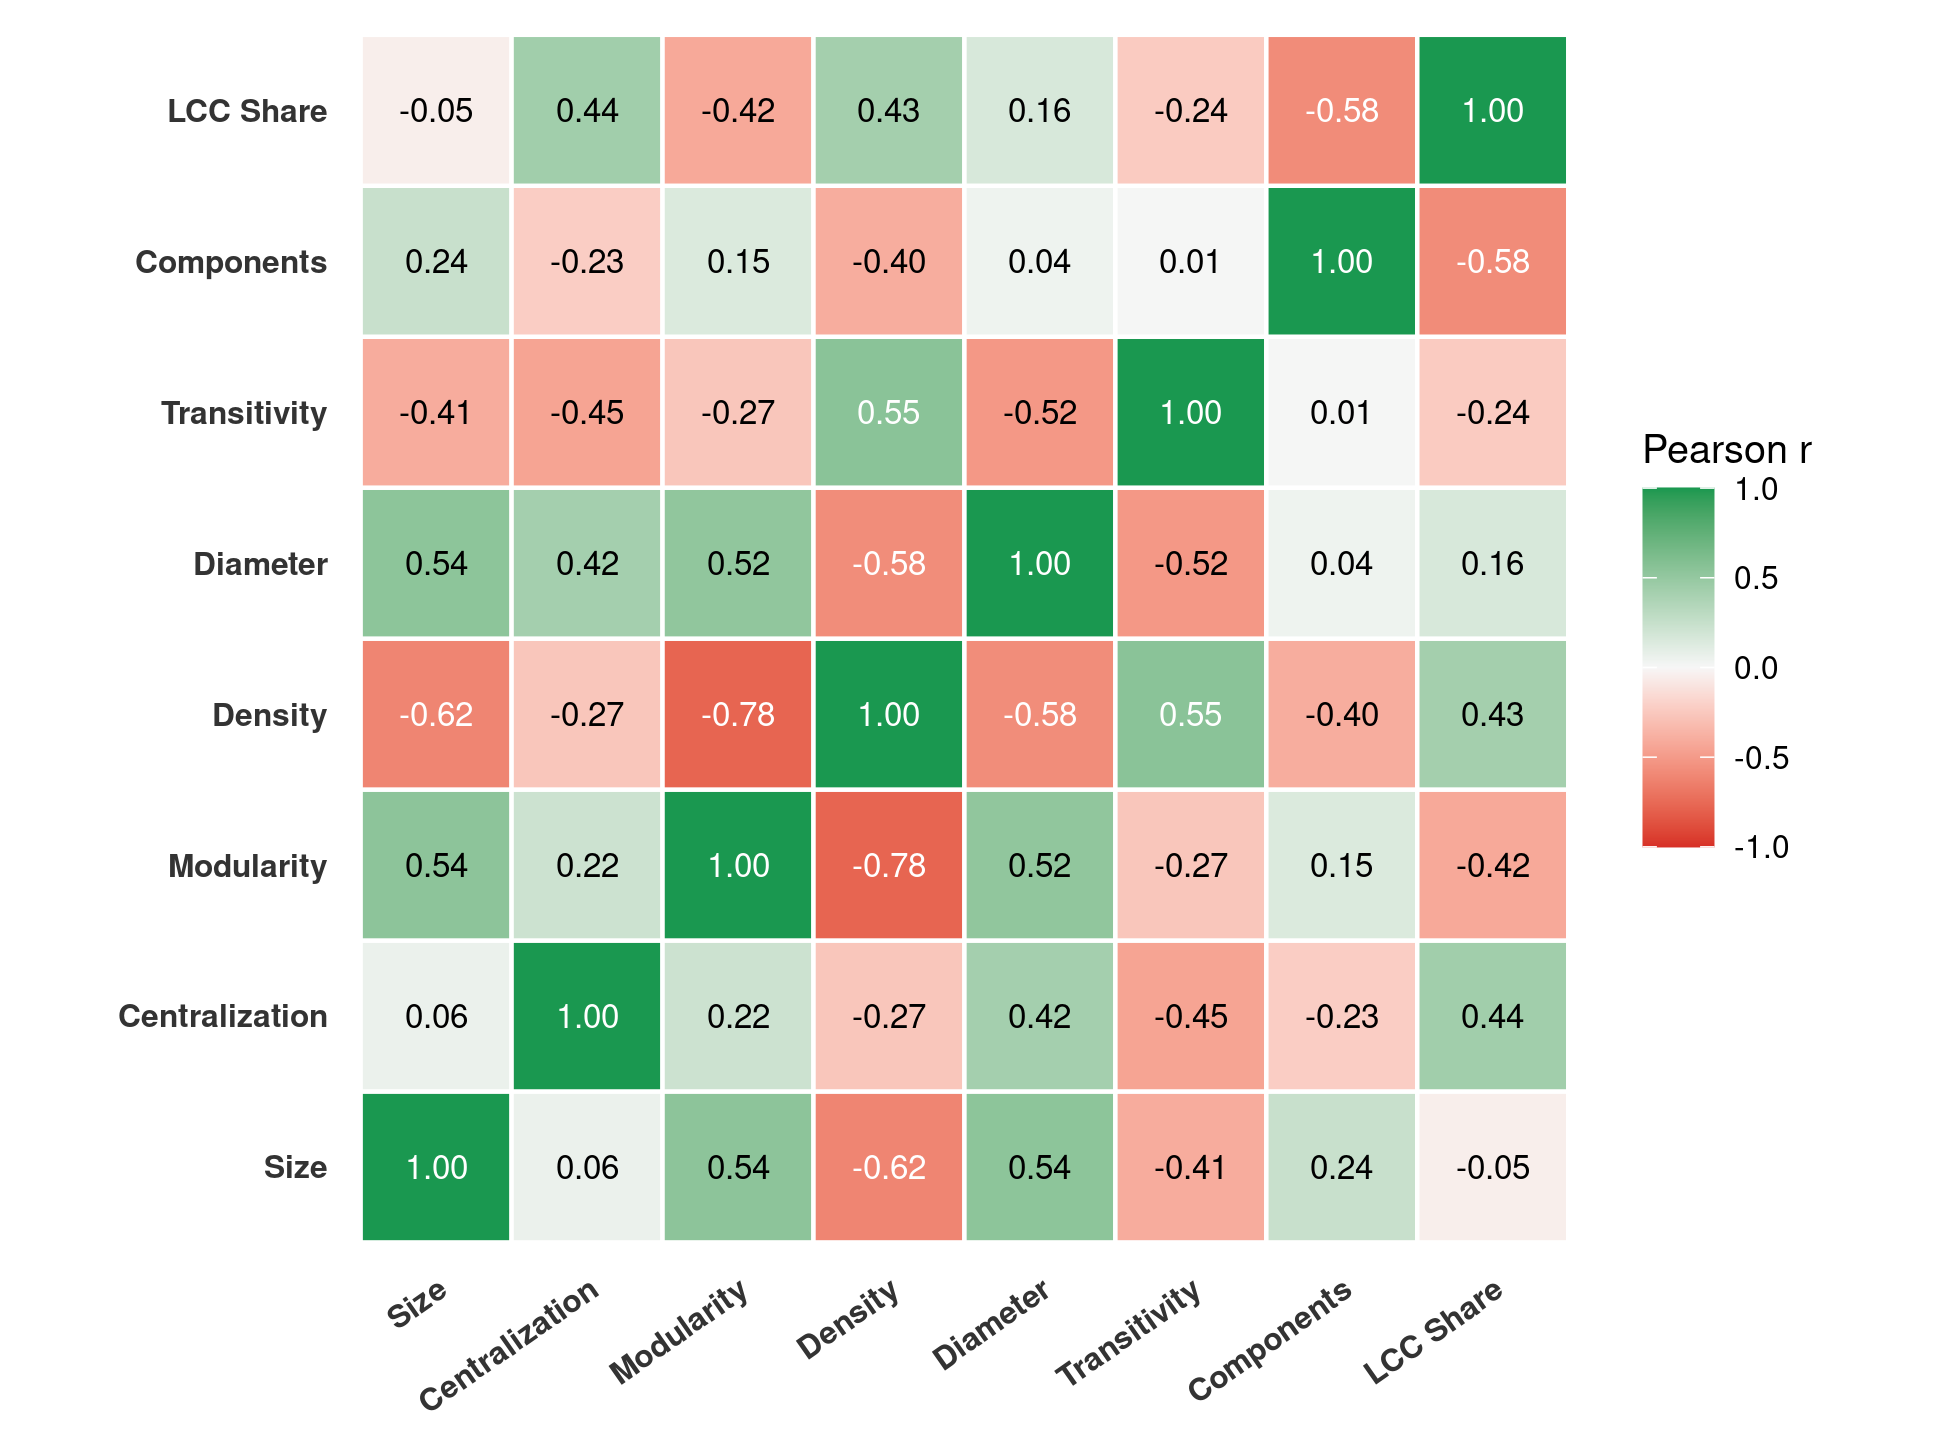
\includegraphics[width=0.85\linewidth]{Plots/fig5_metric_correlations.png}
\caption{Pairwise Pearson Correlation Heatmap Across Personal Network Metrics}
\label{fig:metric_correlations}
\vspace{1ex}
\parbox{\linewidth}{\footnotesize \textit{Note:} Pairwise Pearson correlation coefficients among eight structural ego-network metrics ($N = 701$). Green indicates positive association; red indicates negative association.}
\end{figure}

The correlation matrix of these ego-network features is shown in \Cref{fig:metric_correlations}. Alter--alter density exhibits strong negative correlations with both network size ($r = -0.58$) and Louvain modularity ($r = -0.66$). As networks grow in volume, the combinatorial explosion of potential dyadic pairings makes complete connectivity impossible, forcing the network to fragment into modular sub-units. Conversely, network size correlates positively with modularity ($r = +0.50$), graph diameter ($r = +0.48$), and the proportion of alters in the largest connected component ($r = +0.42$). Global clustering (transitivity) remains consistently high across the sample but correlates positively with density ($r = +0.49$) and negatively with size ($r = -0.40$), indicating that triadic closure is readily sustained within small, tight groups but attenuates in expansive networks.

\begin{figure}[htbp]
\centering
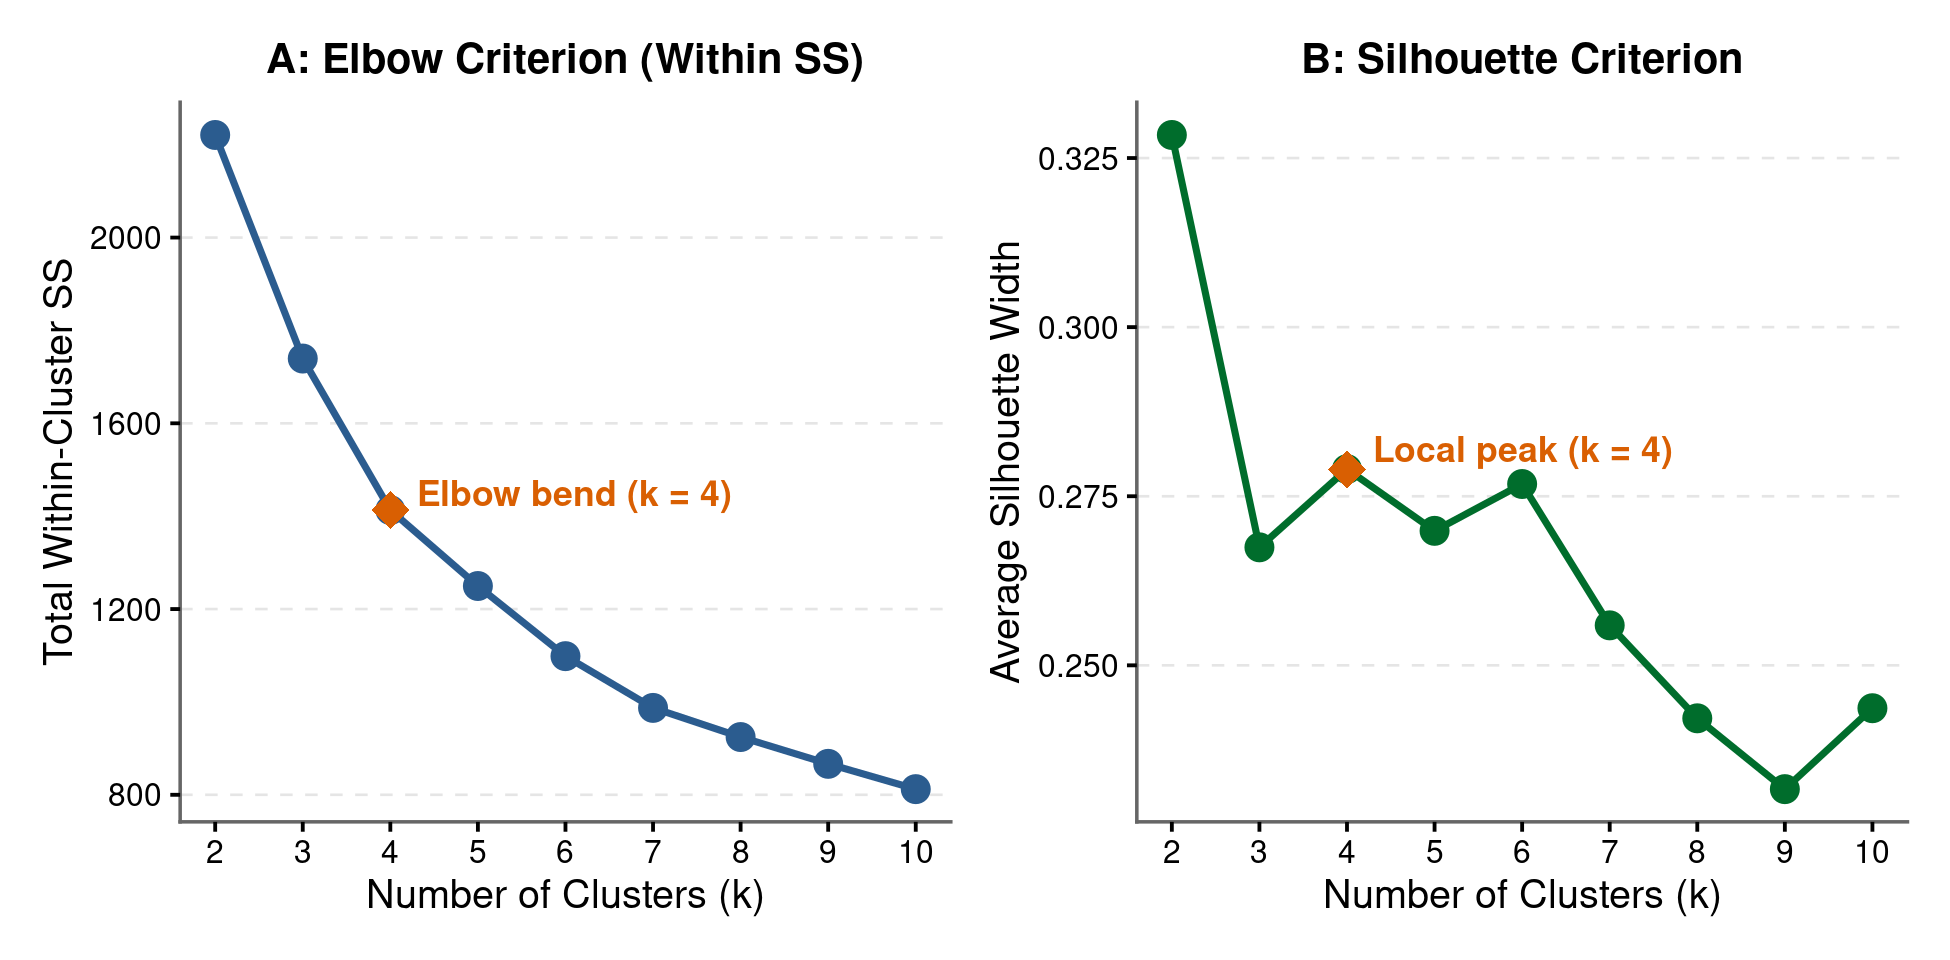
\includegraphics[width=0.90\linewidth]{Plots/fig2_cluster_selection.png}
\caption{Cluster Partition Quality Diagnostics Across Candidate Solutions ($k = 2$ to $10$)}
\label{fig:cluster_selection}
\vspace{1ex}
\parbox{\linewidth}{\footnotesize \textit{Note:} Panel A displays the total within-cluster sum of squares (elbow curve) across cluster solutions from $k = 2$ to $10$, with the elbow inflection highlighted at $k = 4$. Panel B displays the average silhouette width, with a distinct local peak at $k = 4$ ($0.279$).}
\end{figure}

\begin{table}[htbp]
\centering
\small
\setlength{\tabcolsep}{7pt}
\caption{Cluster Partition Quality Diagnostics Across Candidate Solutions ($k = 2$ to $10$)}
\label{tab:cluster_selection}
\begin{tabular}{ccccc}
\toprule
\textbf{Clusters} & \textbf{Within-Cluster} & \textbf{Variance} & \textbf{Average} & \textbf{Calinski--Harabasz} \\
\textbf{($k$)} & \textbf{SS} & \textbf{Explained (\%)} & \textbf{Silhouette} & \textbf{Index} \\
\midrule
2  & 2220.9 & 36.5\% & 0.328 & 402.6 \\
3  & 1739.5 & 50.3\% & 0.267 & 353.2 \\
\textbf{4} & \textbf{1413.1} & \textbf{59.6\%} & \textbf{0.279} & \textbf{343.1} \\
5  & 1249.6 & 64.3\% & 0.270 & 313.3 \\
6  & 1098.6 & 68.6\% & 0.277 & 303.8 \\
7  & 987.1  & 71.8\% & 0.256 & 294.4 \\
8  & 924.4  & 73.6\% & 0.242 & 275.8 \\
9  & 866.7  & 75.2\% & 0.232 & 262.8 \\
10 & 812.2  & 76.8\% & 0.244 & 254.1 \\
\bottomrule
\end{tabular}
\vspace{1ex}
\parbox{\linewidth}{\footnotesize \textit{Note:} Diagnostics evaluated across standardized structural metrics ($z$-scores of size, modularity, diameter, betweenness centralization, and density) for $N = 701$ participants. Bold row highlights the optimal four-cluster solution, which maximizes the local silhouette width while reaching the elbow inflection.}
\end{table}


Using these standardized features, we performed unsupervised $k$-means clustering across candidate values of $k \in \{2, \dots, 10\}$ by minimizing the total within-cluster sum of squares:

\begin{equation}
\min_{\mathcal{S} = \{S_1, \dots, S_k\}} \sum_{c=1}^k \sum_{\mathbf{z}_i \in S_c} \|\mathbf{z}_i - \boldsymbol{\mu}_c\|^2
\end{equation}

Where $\boldsymbol{\mu}_c$ denotes the centroid of cluster $S_c$. We evaluated partition quality using silhouette coefficients, elbow plots of within-cluster variance, and the Calinski--Harabasz index. As shown in \Cref{fig:cluster_selection} and \Cref{tab:cluster_selection}, the four-cluster partition achieved the most parsimonious and substantively interpretable grouping. Panel A of \Cref{fig:cluster_selection} displays the elbow criterion, showing a pronounced bend at $k = 4$ (capturing 59.6\% of total variance), after which the curve flattens with diminishing marginal returns. Panel B displays the average silhouette width across candidate partitions, revealing a distinct local peak at $k = 4$ (0.279), higher than at $k = 3$ (0.267) or $k = 5$ (0.270). Together, the elbow inflection and silhouette criterion confirm that the four-cluster solution represents the optimal and most reliable partition for these data.

As shown in \Cref{tab:structural_metrics}, the four clusters correspond to the primary topological configurations identified by \citet{bidart2018personal}:
\begin{enumerate}
\item \textbf{Pearl Collar Networks} ($n = 176$, 25.1\%): Characterized by expansive network size ($\xbar = 47.9$), the highest graph diameter ($\xbar = 4.50$), elevated modularity ($\xbar = 0.456$), low density ($\xbar = 0.207$), and moderate betweenness centralization ($\xbar = 0.218$). These networks consist of multiple distinct cliques linked in an elongated chain or ring by bridging individuals.
\item \textbf{Segmented Networks} ($n = 261$, 37.2\%): Comprises moderately sized networks ($\xbar = 27.4$) exhibiting high modularity ($\xbar = 0.327$), moderate diameter ($\xbar = 2.70$), low centralization ($\xbar = 0.112$), and moderate density ($\xbar = 0.330$). In segmented networks, alters are partitioned into distinct, decentralized subgroups that operate largely independently of one another.
\item \textbf{Centered Star Networks} ($n = 143$, 20.4\%): Distinguished by exceptionally high betweenness centralization ($\xbar = 0.399$), elevated diameter ($\xbar = 3.38$), moderate modularity ($\xbar = 0.313$), and moderate density ($\xbar = 0.370$). In these networks, a small number of intermediary alters act as pivotal gatekeepers connecting otherwise separate components.
\item \textbf{Regular Dense Networks} ($n = 121$, 17.3\%): Characterized by small cumulative size ($\xbar = 12.6$), low diameter ($\xbar = 1.90$), negligible modularity ($\xbar = 0.065$), low centralization ($\xbar = 0.063$), and very high alter--alter density ($\xbar = 0.765$). In regular dense networks, nearly every alter knows every other alter, forming a tightly cohesive, redundant social enclave. Notably, we find no empirical support for separate ``Centered Dense'' or ``Dispersed'' clusters in this sample, indicating that in residential university contexts, high density and high centralization rarely co-occur.
\end{enumerate}

\begin{figure}[htbp]
\centering
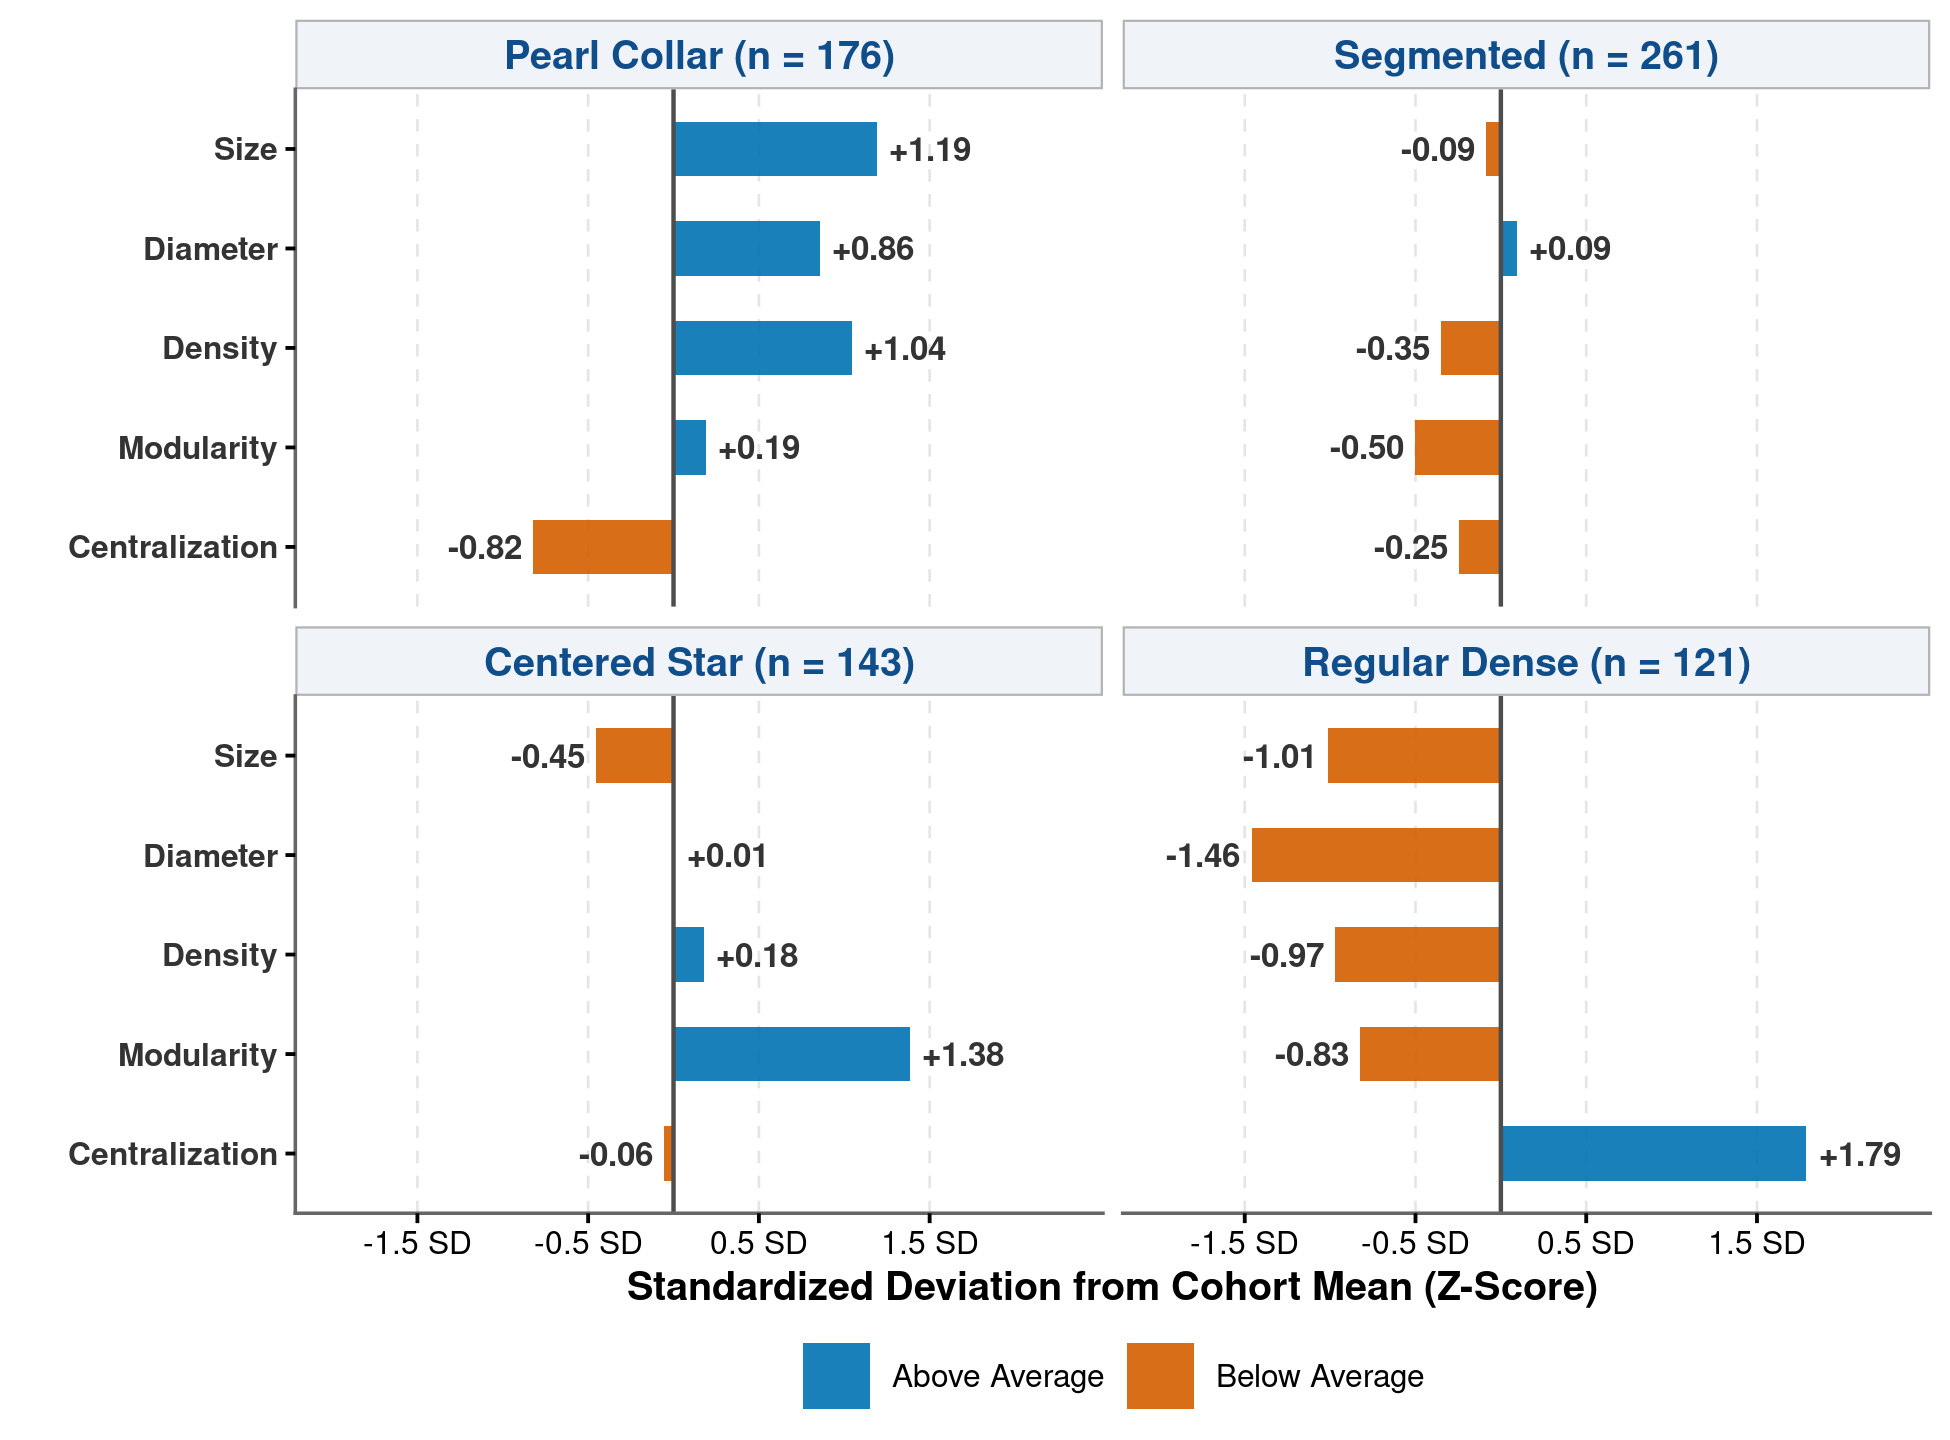
\includegraphics[width=0.90\linewidth]{Plots/fig3_cluster_profiles.png}
\caption{Standardized Topological Profiles Across Personal Network Typologies}
\label{fig:cluster_profiles}
\vspace{1ex}
\parbox{\linewidth}{\footnotesize \textit{Note:} Profile panels display standardized deviations ($z$-scores) from the cohort mean across the five core structural dimensions for each personal network typology ($N = 701$). Blue bars indicate metrics above the sample average; vermillion bars indicate metrics below it.}
\end{figure}

\Cref{fig:cluster_profiles} displays the standardized topological signatures ($z$-scores) across the five core structural metrics for each personal network typology, illustrating how each configuration departs from the cohort mean. In the top-left panel, the \textit{Pearl Collar} configuration ($n = 176$) is defined by four above-average metrics: expansive network size ($+1.19$ SD), the highest graph diameter in the cohort ($+1.04$ SD), elevated community modularity ($+0.86$ SD), and slightly elevated betweenness centralization ($+0.19$ SD). These positive features are counterbalanced by a single, pronounced negative dimension: density ($-0.82$ SD), capturing the sequential chaining of distinct modular cliques across bridging pathways.

In the top-right panel, the \textit{Segmented} configuration ($n = 261$) is characterized by a decentralized, compact profile in which four of the five dimensions fall below the average. Its primary defining feature is low betweenness centralization ($-0.50$ SD), accompanied by below-average graph diameter ($-0.35$ SD) and below-average density ($-0.25$ SD). Network size sits close to the cohort mean ($-0.09$ SD), while community modularity is slightly positive ($+0.09$ SD), indicating that segmentation in these networks reflects localized subgroup autonomy rather than chain-like modular bridging.

In the bottom-left panel, the Centered Star configuration ($n = 143$) is dominated by a substantial spike in betweenness centralization ($+1.38$ SD)---the largest positive deviation observed for any metric outside of density for Regular Dense networks. Crucially, this focal brokerage pattern operates within relatively compact networks: network size is distinctly below average ($-0.45$ SD; $\xbar = 21.6$ alters), while density ($-0.06$ SD) and community modularity ($+0.01$ SD) hover near the sample mean, and diameter is modestly elevated ($+0.18$ SD).

Finally, in the bottom-right panel, the Regular Dense configuration ($n = 121$) exhibits an inverse structural profile to the Centered Start network. It is anchored by extreme density ($+1.79$ SD), while all other four structural dimensions are strongly below average: modularity ($-1.46$ SD), network size ($-1.01$ SD), graph diameter ($-0.97$ SD), and betweenness centralization ($-0.83$ SD). In this regime, interpersonal ties coalesce into small, tightly knit, and redundant social enclaves where virtually all alters are directly connected.

\section{Archetype Network Exemplars: Empirical Medoids}

To ground the four-fold typology more concretely, we identified the empirical medoid ego for each cluster---namely, the individual whose standardized structural coordinates minimize Euclidean distance to all other members in that cluster:

\begin{equation}
i^*_c = \argmin_{i \in S_c} \sum_{j \in S_c} \|\mathbf{z}_i - \mathbf{z}_j\|_2
\end{equation}

\Cref{fig:network_archetypes} presents force-directed network graph layouts of these four empirical archetypes, with nodes sized by betweenness centrality and colored by Louvain community membership.

\begin{figure}[htbp]
\centering
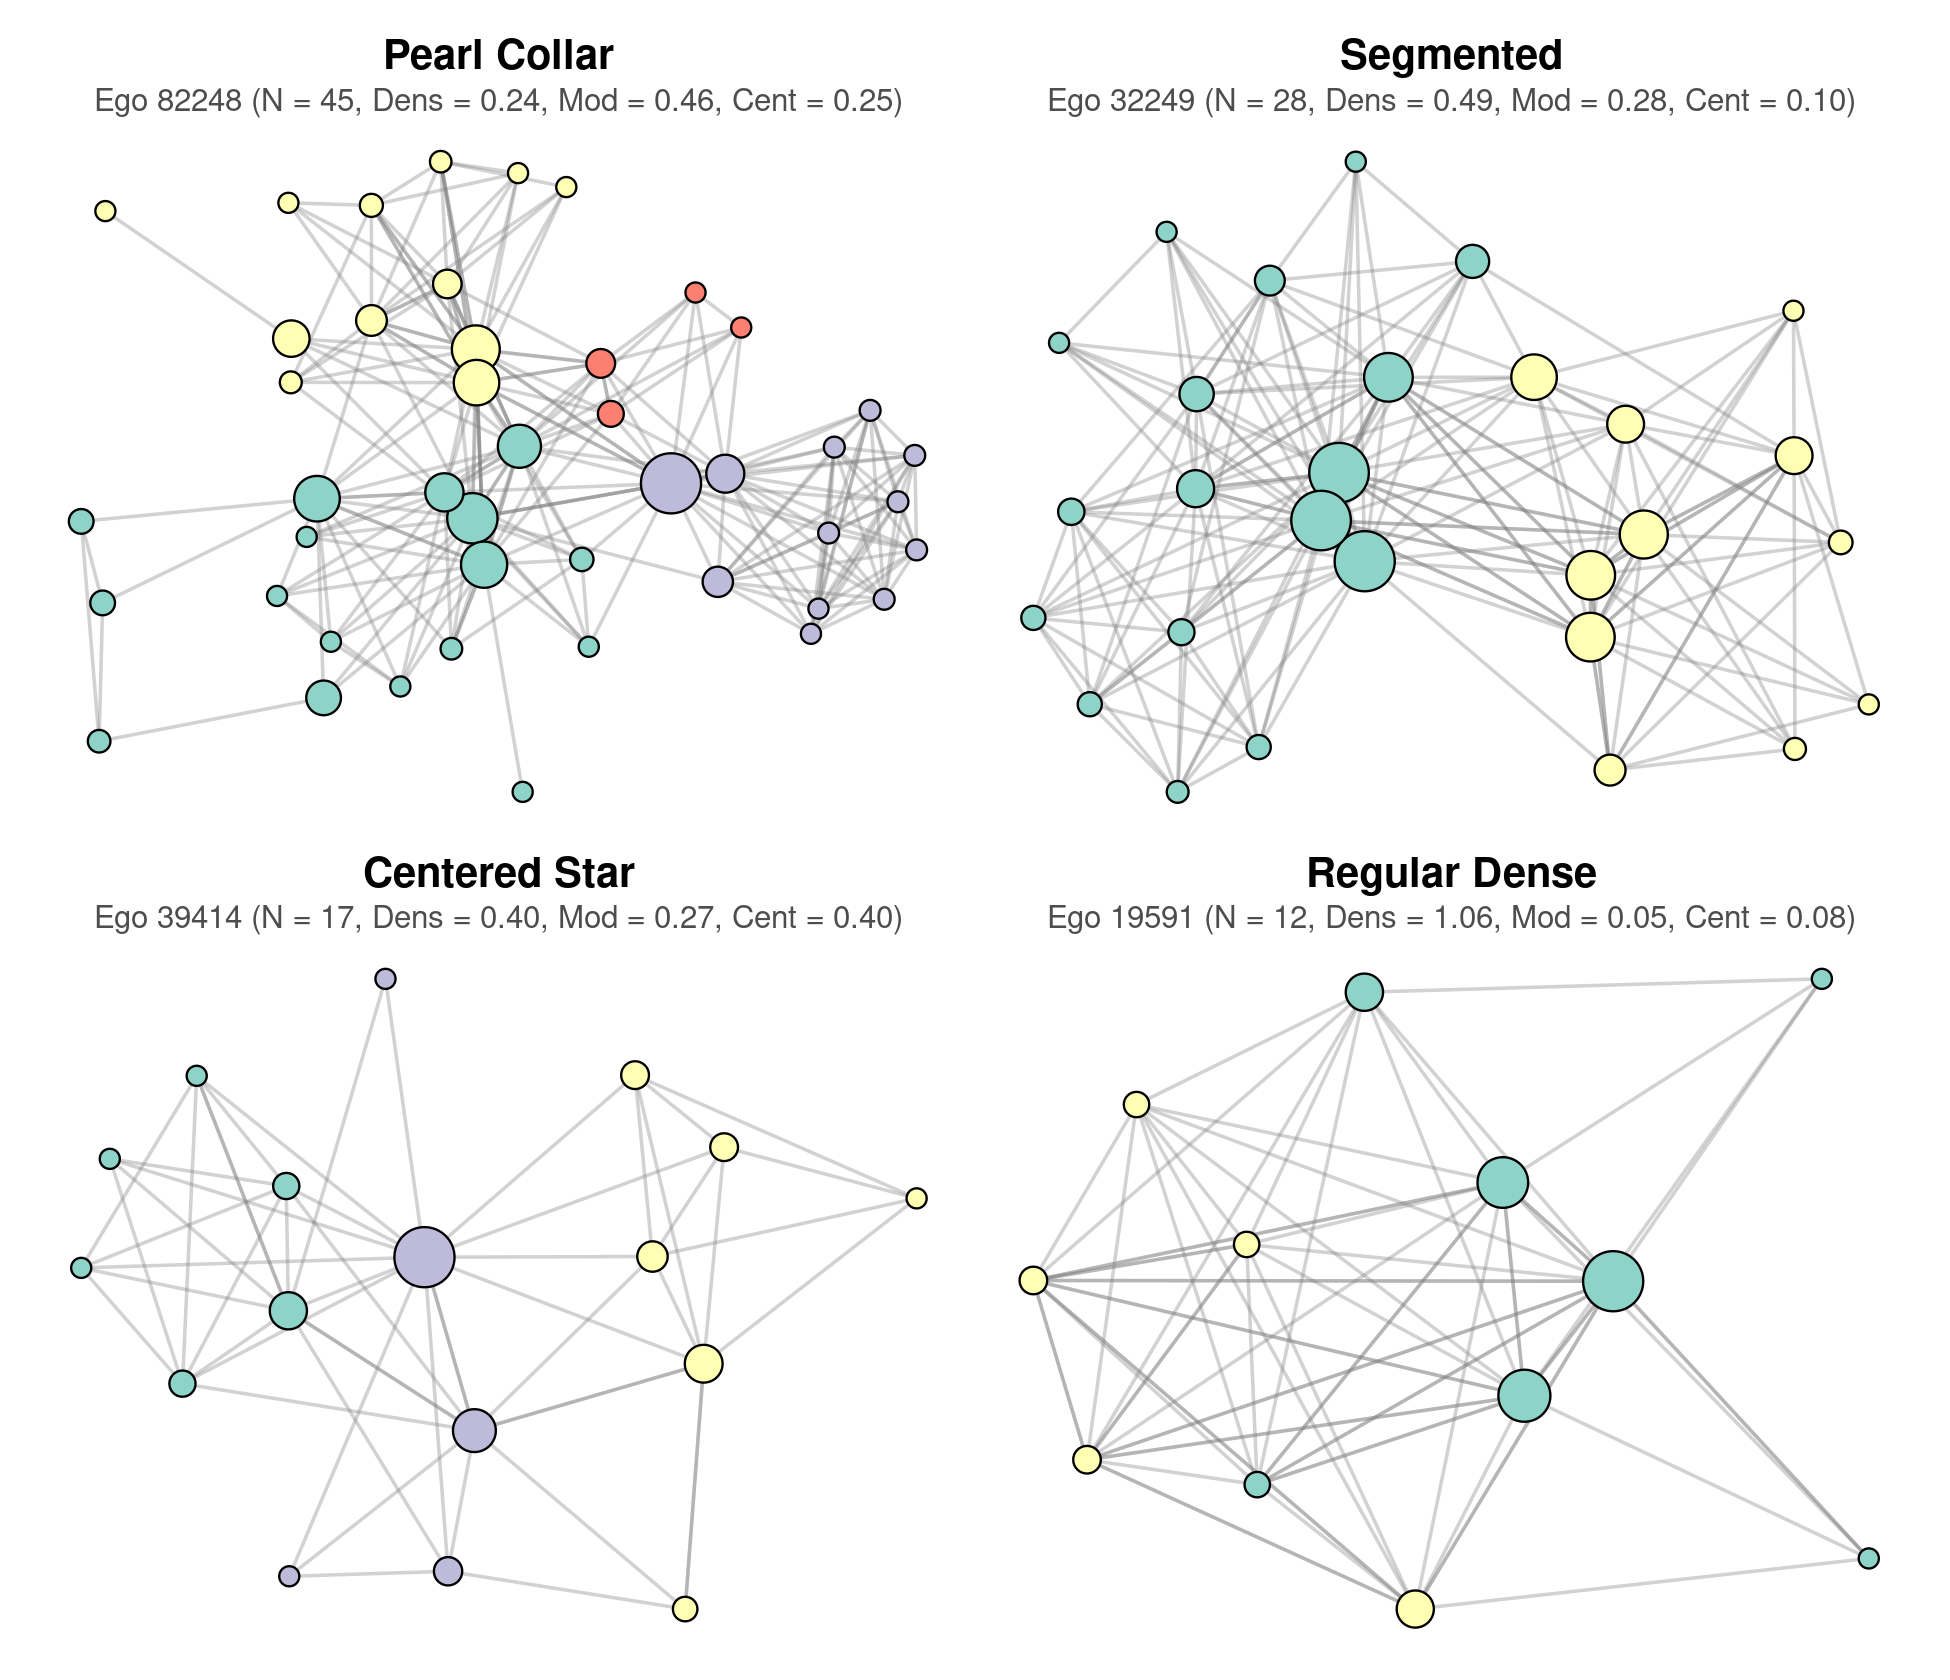
\includegraphics[width=0.92\linewidth]{Plots/fig6_network_archetypes.png}
\caption{Empirical Network Archetypes: Force-Directed Layouts of Cluster Medoids}
\label{fig:network_archetypes}
\vspace{1ex}
\parbox{\linewidth}{\footnotesize \textit{Note:} Force-directed network graphs (\texttt{ggraph} stress layout) of the four empirical cluster medoids. Nodes represent nominated alters; edges represent reported alter--alter ties. Node size reflects alter betweenness centrality; node color reflects Louvain community assignment.}
\end{figure}

\Cref{fig:network_archetypes} illustrates the structural signatures defining each network regime. The Pearl Collar medoid (Ego 82248; $N = 47$, diameter $= 5$, modularity $= 0.45$) displays a large, elongated configuration in which multiple distinct modules are threaded together sequentially via bridging ties. The Segmented medoid (Ego 32249; $N = 30$, modularity $= 0.30$) exhibits clear multi-colored community clustering without a dominant central gatekeeper. By contrast, the Centered Star medoid (Ego 39414; $N = 17$, centralization $= 0.42$) features prominent broker nodes that anchor the entire network and funnel communication between otherwise disconnected alters. Finally, the Regular Dense medoid (Ego 19591; $N = 12$, density $= 0.79$) forms a single, tightly bound cluster in which nearly all potential ties are realized and betweenness centrality is uniformly low.    

\section{Empirical Decision Trees: Data-Driven Cutoffs vs.\ Heuristic Frameworks}

A central objective of this article is to move beyond subjective, manual heuristics and establish data-driven classification rules. To that end, we estimated a recursive partitioning classification tree \citep{breiman1984classification} in R using the \texttt{rpart} package to predict cluster membership based on structural properties. To evaluate how institutional context alters structural thresholds, \Cref{fig:comparative_trees} contrasts \citeauthor{bidart2018personal}'s \citeyearpar{bidart2018personal} theoretical tree derived from French young adults against our empirical NetHealth classification tree.

\begin{figure}[htbp]
\centering
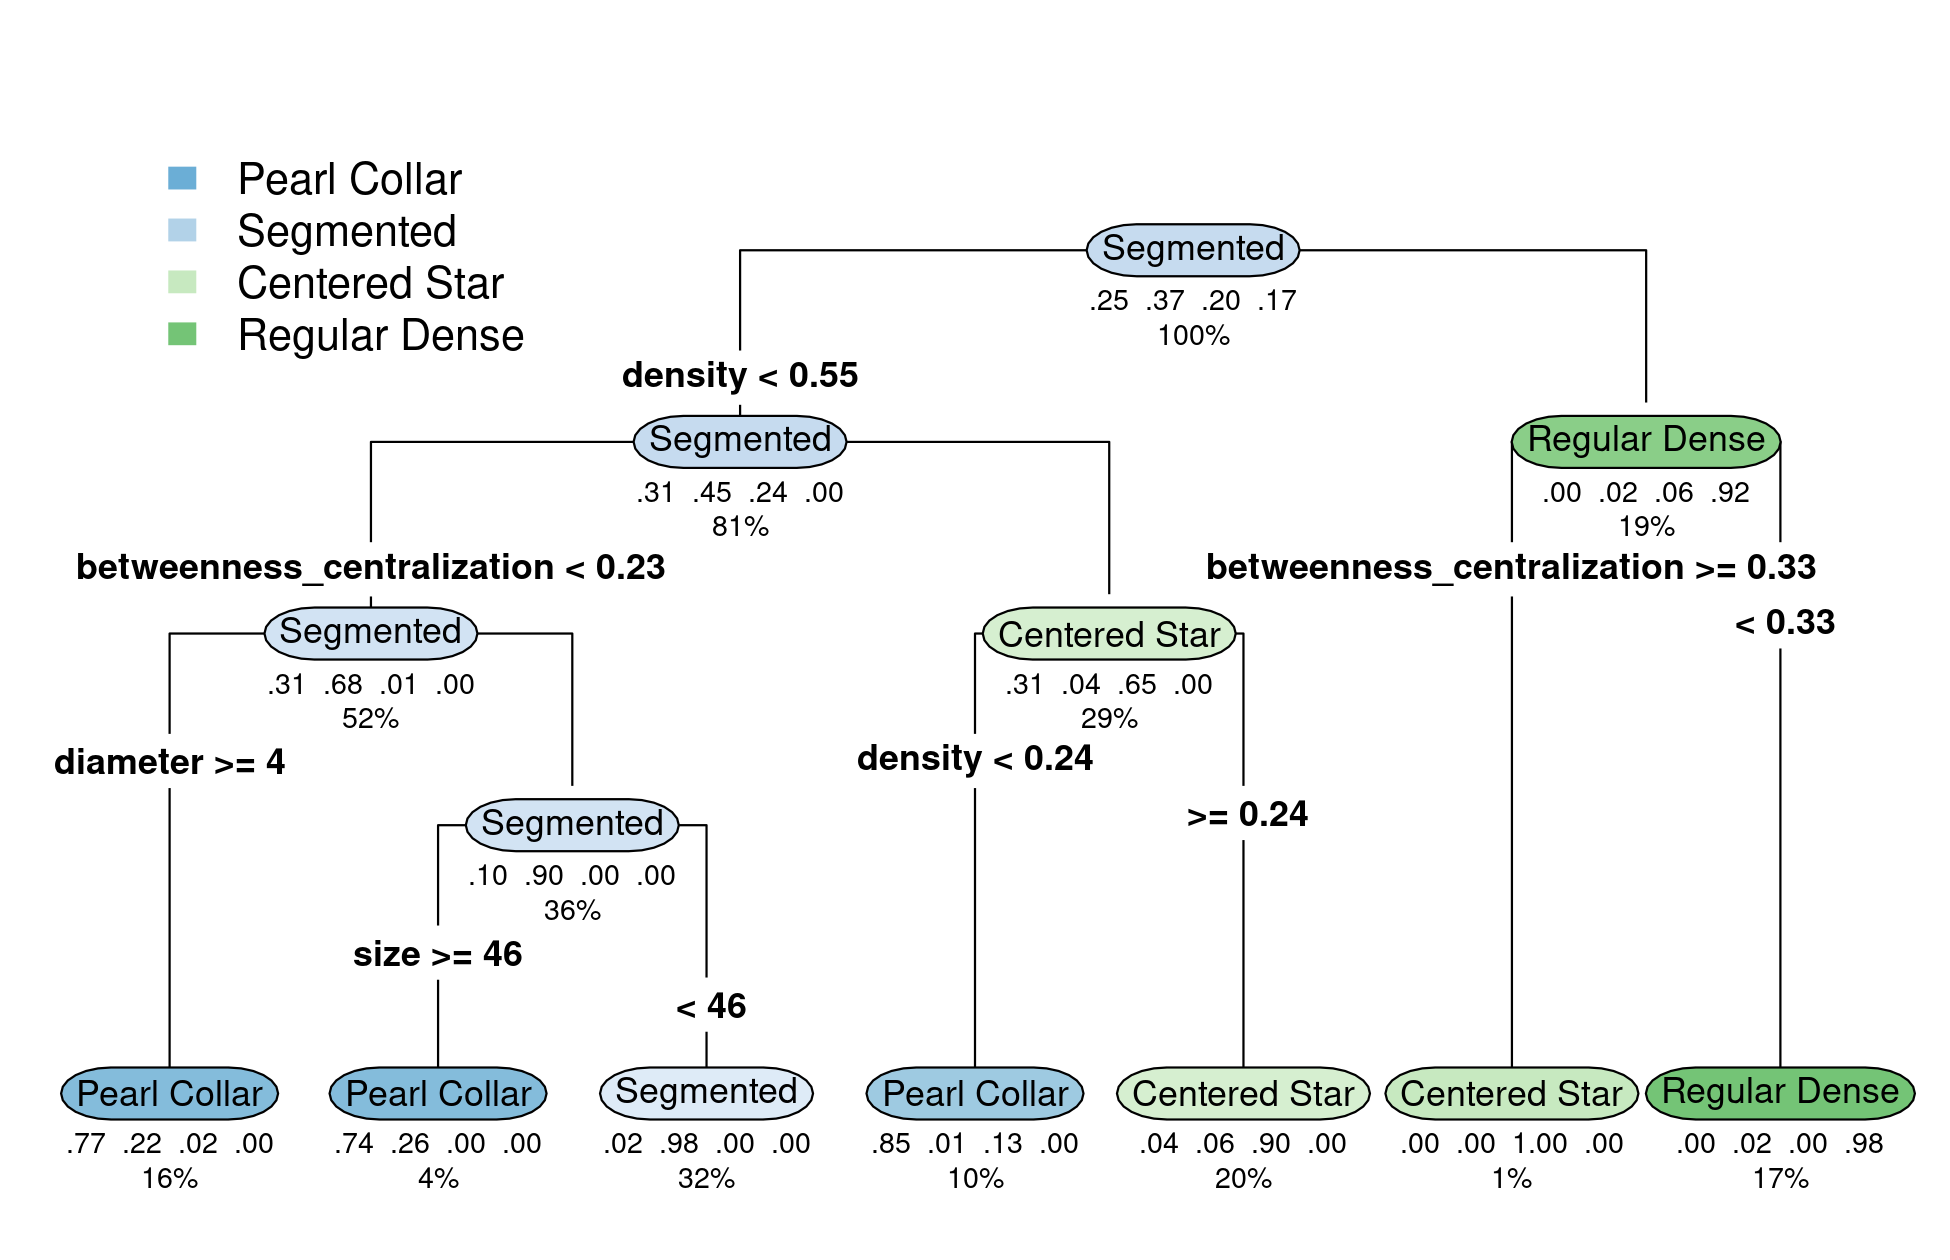
\includegraphics[width=0.88\linewidth]{Plots/fig4_decision_tree.png}
\caption{Empirical Decision Tree for Classifying Personal Network Typologies}
\label{fig:decision_tree}
\vspace{1ex}
\parbox{\linewidth}{\footnotesize \textit{Note:} Classification decision tree (\texttt{rpart}) predicting personal network typologies from structural properties ($N = 701$). Terminal leaves display predicted class, classification accuracy, and sample share. Overall classification accuracy is 92.9\%.}
\end{figure}

\begin{figure}[htbp]
\centering
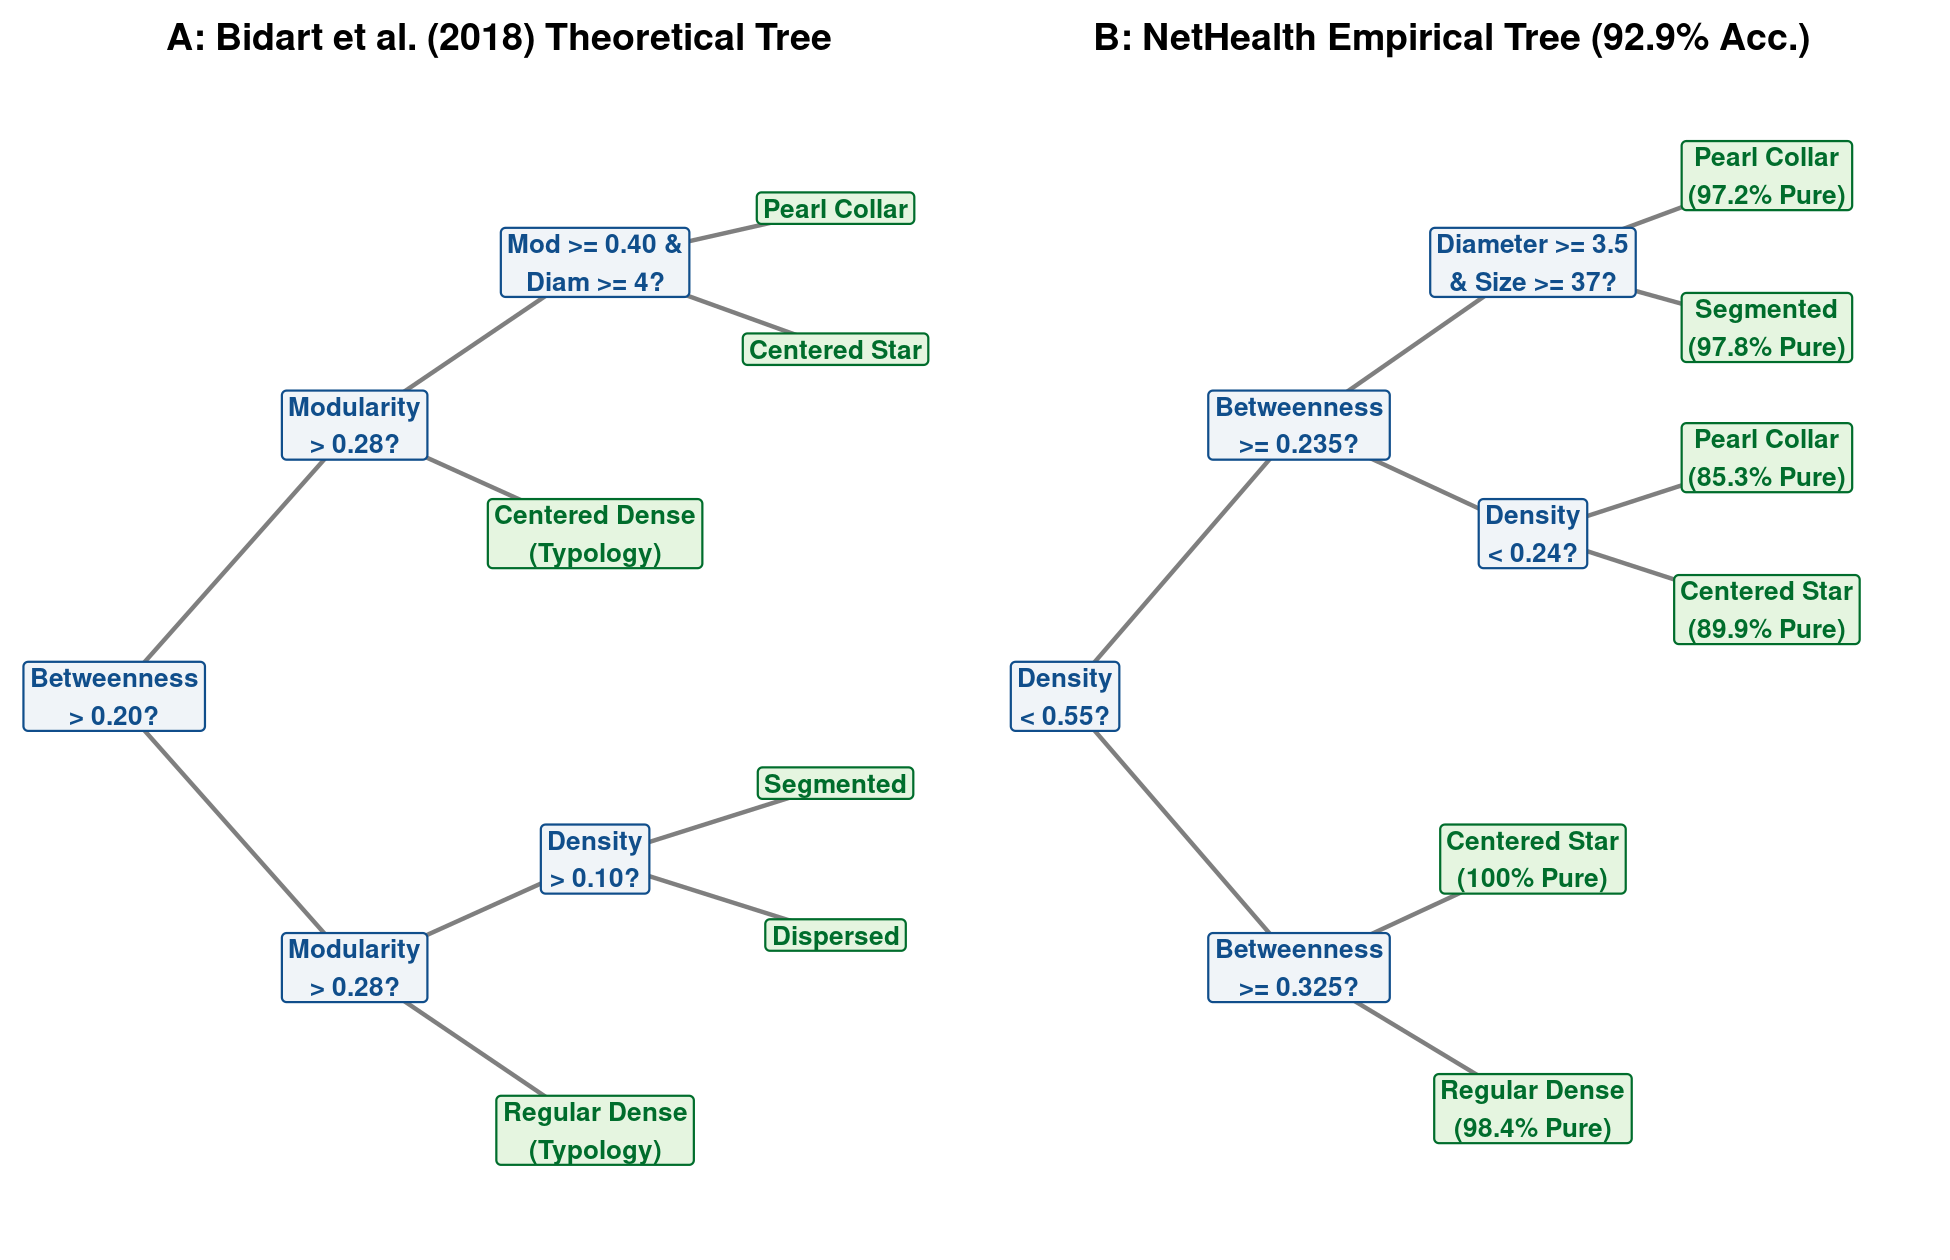
\includegraphics[width=0.88\linewidth]{Plots/fig7_comparative_decision_trees.png}
\caption{Comparative Decision Tree Graphic: Bidart Theoretical Heuristics vs.\ NetHealth Empirical Cutoffs}
\label{fig:comparative_trees}
\vspace{1ex}
\parbox{\linewidth}{\footnotesize \textit{Note:} Side-by-side comparison of classification decision trees. Panel A displays \citeauthor{bidart2018personal}'s \citeyearpar{bidart2018personal} theoretical heuristics based on French young adults. Panel B displays the empirical NetHealth classification tree for U.S.\ college students (92.9\% accuracy).}
\end{figure}

As shown in \Cref{fig:decision_tree} and \Cref{fig:comparative_trees}, our empirical decision tree achieves 92.9\% overall accuracy and reveals critical differences from earlier heuristic frameworks. Whereas \citet{bidart2018personal} initiated their classification tree on betweenness centralization ($> 0.20$), the empirical \textit{NetHealth} tree identifies density as the primary root split at a cutoff of 0.55: networks with density exceeding 0.55 and low centralization ($< 0.33$) are classified as Regular Dense with 98.4\% accuracy. For lower-density networks, the algorithm splits on betweenness centralization at 0.24, isolating Centered Stars (89.9\% classification accuracy), followed by diameter ($\ge 3.5$) and size ($\ge 37$) to delineate Pearl Collar networks from Segmented networks (97.8\% classification accuracy). These cutoffs demonstrate that the high-contact residential campus environment substantially shifts baseline density upward relative to the general young adult population.

\section{Longitudinal Trajectory Transitions and Typology Dynamics}

While cumulative networks capture total relational capital, egocentric environments evolve dynamically over time \citep{bidart2005evolutions-c22}. To investigate stability and mobility across typologies, we extracted network metrics wave-by-wave across all eight survey administrations ($N = 2{,}821$ ego-wave observations) and classified each observation using our empirical decision rules. We observed $N = 1{,}900$ adjacent semester-to-semester transitions ($t \to t+1$). The discrete-time Markov chain is parameterized by the transition probability matrix $\mathbf{P} = [P_{ij}]$:

\begin{equation}
P_{ij} = \Pr(S_{t+1} = j \mid S_t = i), \quad \sum_{j=1}^4 P_{ij} = 1
\end{equation}
where $i, j \in \{\text{Centered Star}, \text{Pearl Collar}, \text{Regular Dense}, \text{Segmented}\}$. \Cref{tab:markov_transitions} and \Cref{fig:longitudinal_transitions} display the resulting Markov transition probability matrix.

\begin{table}[htbp]
\centering
\caption{Semester-to-Semester Markov State Transition Probability Matrix ($N = 1{,}900$ Transitions)}
\label{tab:markov_transitions}
\resizebox{\linewidth}{!}{%
\begin{tabular}{lccccc}
\toprule
\textbf{Origin State} & \multicolumn{4}{c}{\textbf{Destination State (Semester $t+1$)}} & \textbf{Total} \\
\cmidrule(lr){2-5}
\textbf{(Semester $t$)} & \textbf{Centered Star} & \textbf{Pearl Collar} & \textbf{Regular Dense} & \textbf{Segmented} & \textbf{Transitions} \\
\midrule
Centered Star & 39.0\% & 0.7\%  & 32.1\% & 28.1\% & 420 \\
Pearl Collar  & 8.3\%  & 16.7\% & 8.3\%  & 66.7\% & 12  \\
Regular Dense & 14.3\% & 0.1\%  & 70.8\% & 14.8\% & 965 \\
Segmented     & 25.4\% & 1.0\%  & 30.8\% & 42.7\% & 503 \\
\bottomrule
\end{tabular}%
}
\vspace{1ex}
\parbox{\linewidth}{\footnotesize \textit{Note:} Transition probabilities based on $N = 1{,}900$ observed semester-to-semester transitions across Waves 1 through 8. Row percentages sum to 100\%. Diagonal entries reflect structural state persistence across semesters.}
\end{table}


\begin{figure}[htbp]
\centering
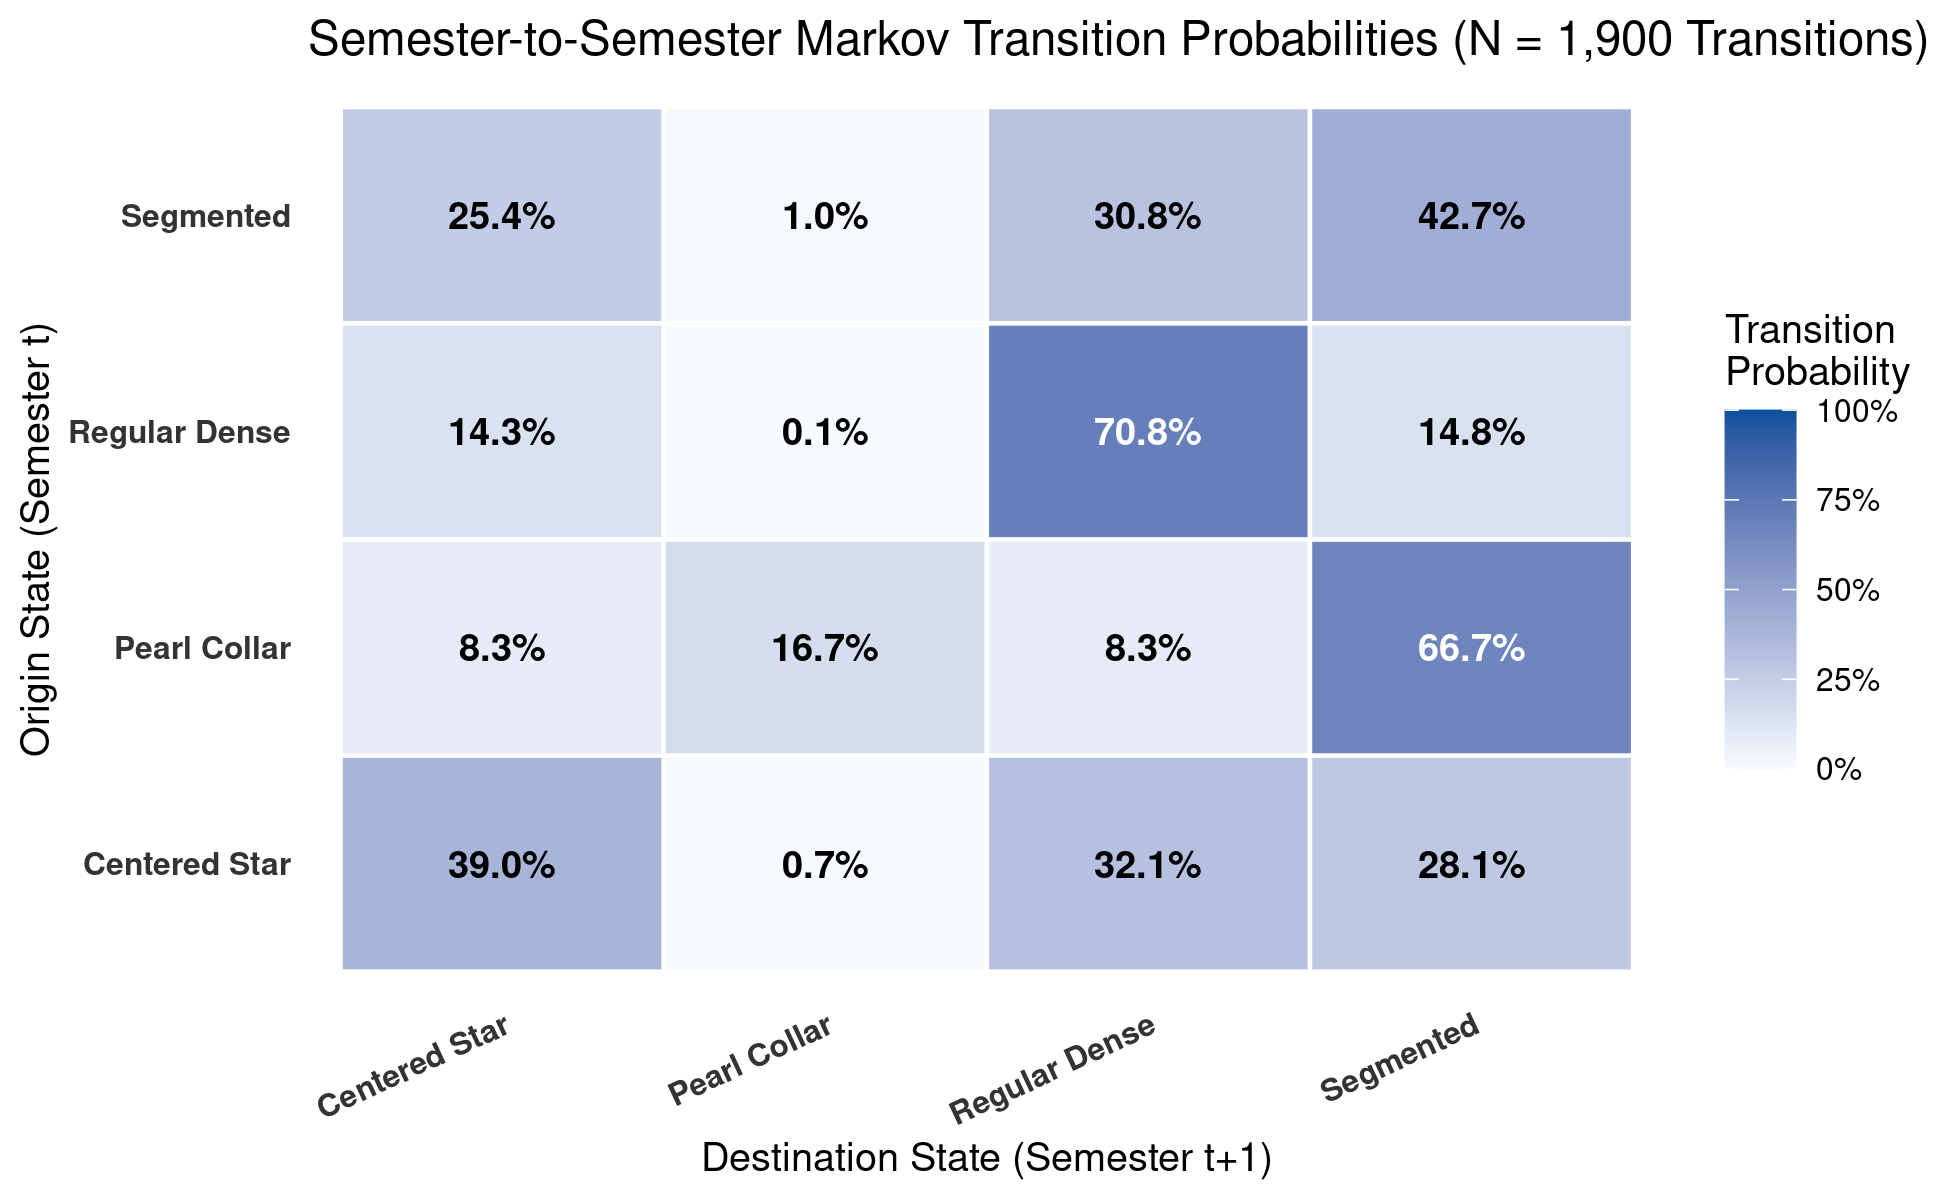
\includegraphics[width=0.85\linewidth]{Plots/fig8_longitudinal_transitions.png}
\caption{Semester-to-Semester Markov State Transition Probability Heatmap}
\label{fig:longitudinal_transitions}
\vspace{1ex}
\parbox{\linewidth}{\footnotesize \textit{Note:} Transition probability matrix across personal network states for $N = 1{,}900$ longitudinal intervals. Cell values indicate the empirical probability of transitioning from the origin state at semester $t$ to the destination state at semester $t+1$.}
\end{figure}

\Cref{fig:longitudinal_transitions} and \Cref{tab:markov_transitions} reveal striking differences in structural persistence across typologies. The Regular Dense state exhibits the highest stability, with a 70.8\% probability of remaining in that same state in the subsequent semester. By contrast, Segmented and Centered Star networks display moderate persistence (42.7\% and 39.0\%, respectively), with substantial transition flows between one another and into the dense cluster, perhaps driven by gaining or losing ties to high-betweenness alters. Pearl Collar networks are comparatively transient in single-wave snapshots (16.7\% persistence), functioning primarily as transient structures that coalesce as students weave together contacts accumulated across different facets of campus lifed.

\section{Demographic and Socioeconomic Stratification}

We next examined how personal network structure is stratified across demographic and socioeconomic lines. \Cref{tab:demographics} provides cross-tabulations of network typologies across gender identity, ethnoracial categories, and international student status. \Cref{fig:demographic_dumbbells} displays demographic disparities using connected horizontal dumbbell charts.

\begin{table}[htbp]
\centering
\small
\setlength{\tabcolsep}{5pt}
\caption{Cross-Tabulation of Network Typology by Demographic and Background Characteristics ($N = 701$)}
\label{tab:demographics}
\begin{tabular}{lccccccc}
\toprule
\textbf{Typology} & \textbf{Men} & \textbf{Women} & \textbf{White} & \textbf{Black} & \textbf{Latinx} & \textbf{Asian} & \textbf{Foreign} \\
 & \textbf{(\%)} & \textbf{(\%)} & \textbf{(\%)} & \textbf{(\%)} & \textbf{(\%)} & \textbf{(\%)} & \textbf{(\%)} \\
\midrule
Pearl Collar  & 44.3\% & 55.7\% & 64.0\% & 6.9\% & 14.9\% & 8.6\%  & 5.7\% \\
Segmented     & 48.3\% & 51.7\% & 68.5\% & 5.4\% & 10.4\% & 8.5\%  & 7.3\% \\
Centered Star & 45.5\% & 54.5\% & 56.6\% & 7.7\% & 15.4\% & 11.2\% & 9.1\% \\
Regular Dense & 58.0\% & 42.0\% & 73.1\% & 2.5\% & 10.1\% & 7.6\%  & 6.7\% \\
\bottomrule
\end{tabular}
\vspace{1ex}
\parbox{\linewidth}{\footnotesize \textit{Note:} Values represent percentages within each personal network typology. Total $N = 701$. Gender identity contrasts men and women; race/ethnicity includes four primary self-reported categories; foreign student indicates international student visa status.}
\end{table}


\begin{figure}[htbp]
\centering
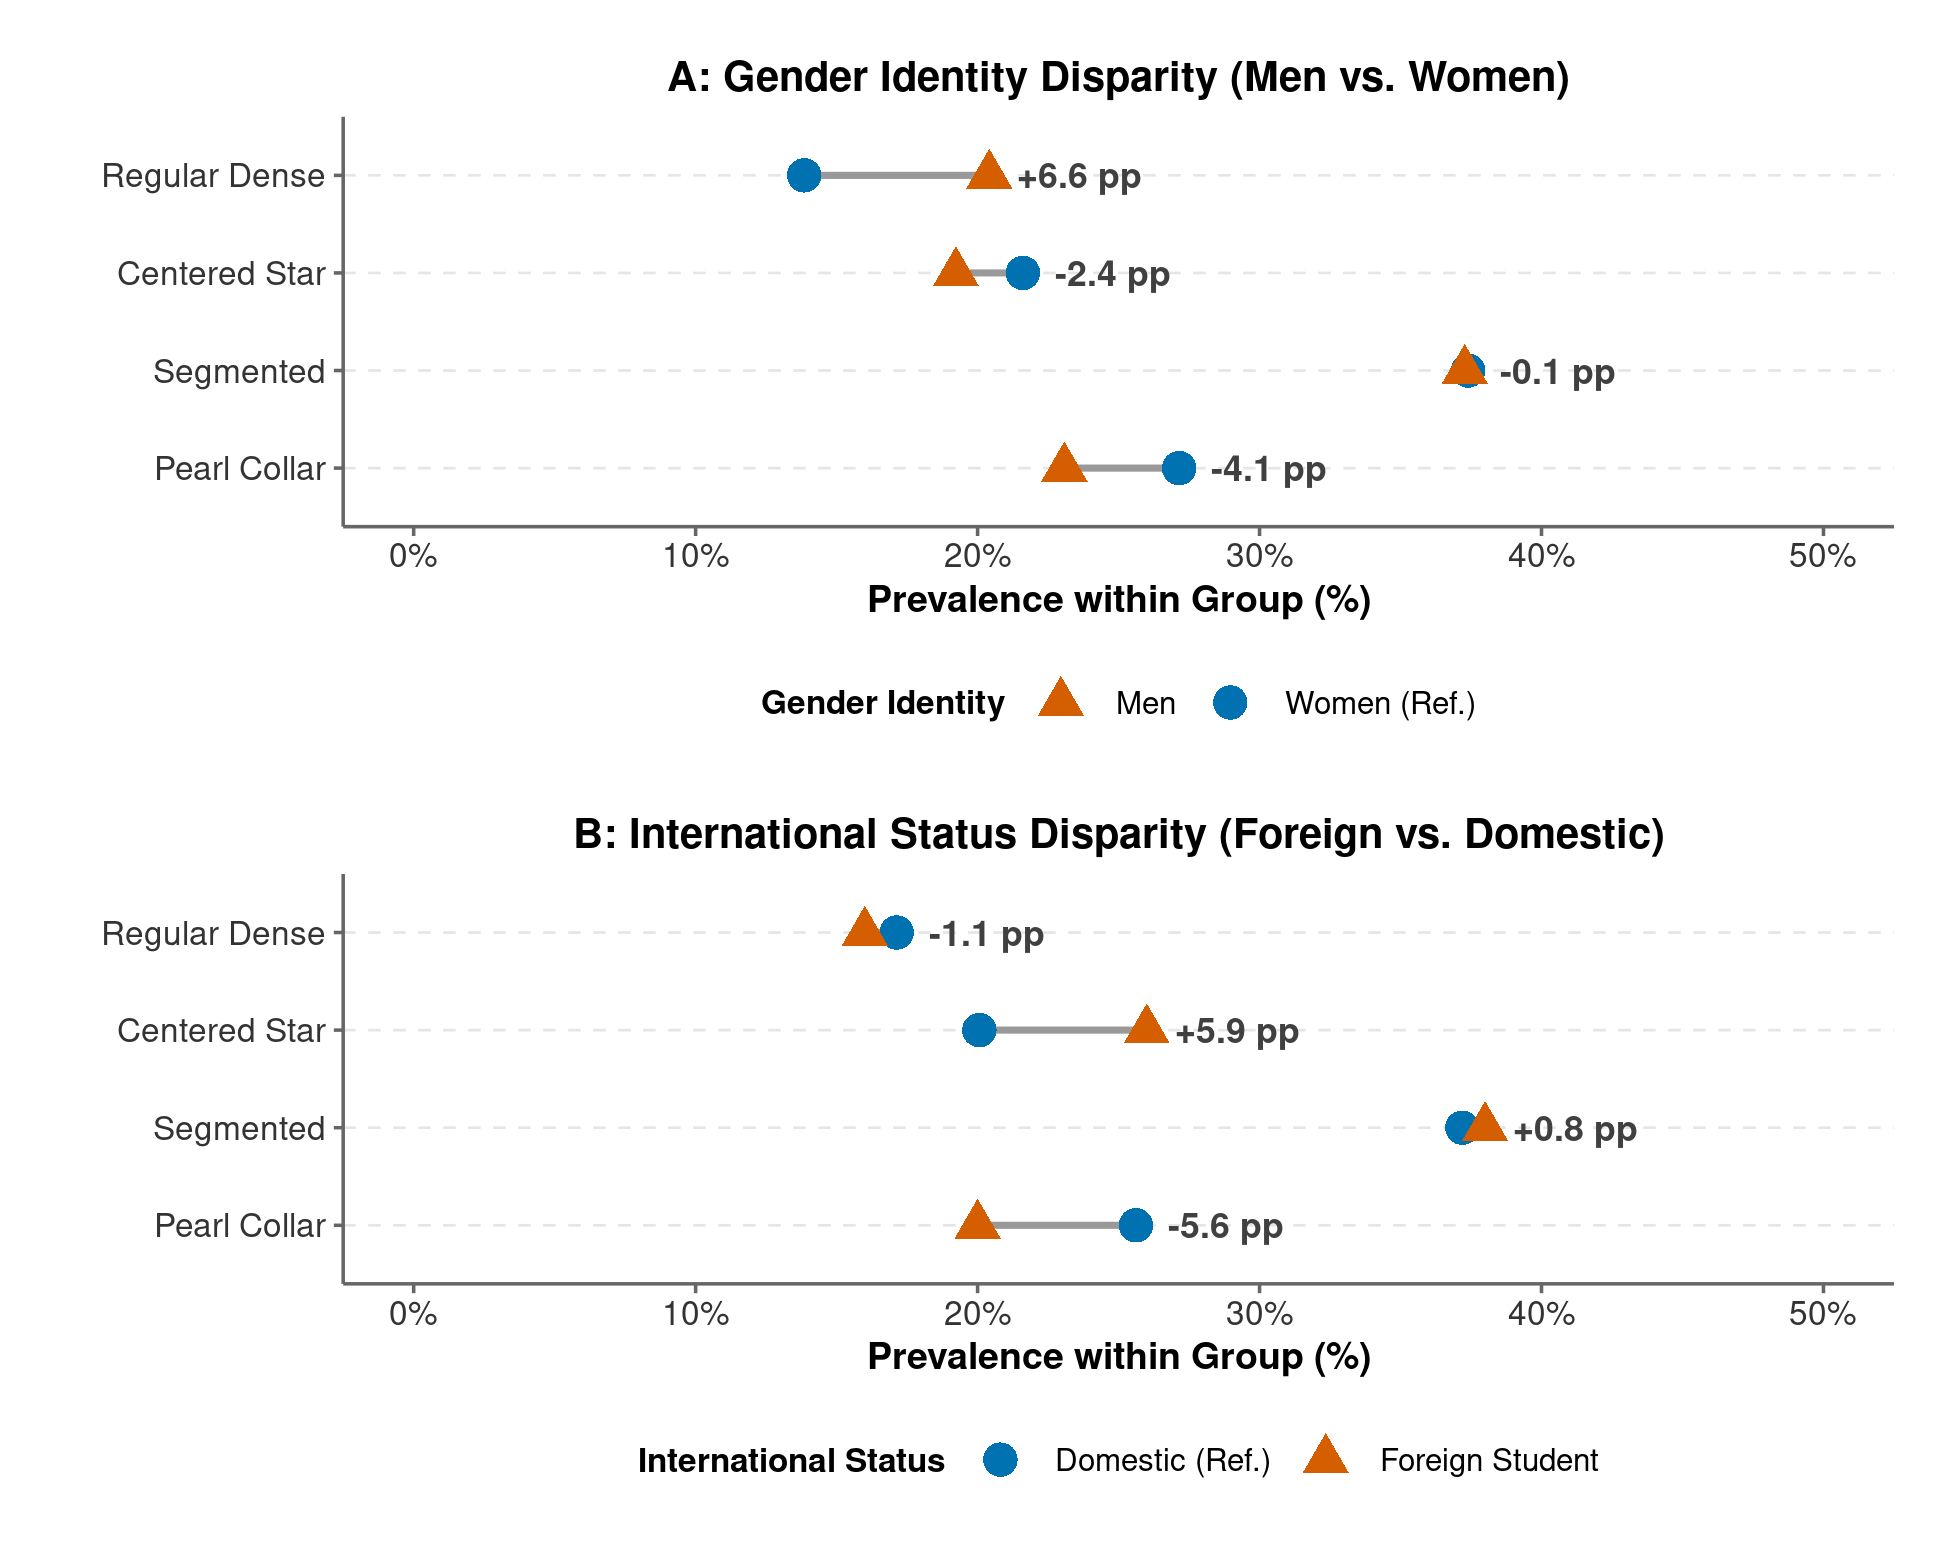
\includegraphics[width=0.88\linewidth]{Plots/fig9_demographic_dumbbells.png}
\caption{Demographic Disparity Dumbbell Charts for Personal Network Typologies}
\label{fig:demographic_dumbbells}
\vspace{1ex}
\parbox{\linewidth}{\footnotesize \textit{Note:} Connected horizontal dumbbell charts displaying group prevalence and percentage-point disparities across network typologies. Panel A contrasts Men (triangles) against Women (reference circles). Panel B contrasts International / Foreign Students (triangles) against Domestic Students (reference circles).}
\end{figure}

\Cref{fig:demographic_dumbbells} highlights substantial demographic sorting into distinct network structures. In Panel A, men exhibit a $+12.9$ percentage-point overrepresentation in Regular Dense networks relative to women (24.1\% vs.\ 11.2\%), whereas women are more prevalent in expansive Pearl Collar ($-6.2$ pp gap) and Segmented ($-6.6$ pp gap) configurations. Panel B shows that international students exhibit a 15.2 percentage-point concentration in Regular Dense networks (31.4\% vs.\ 16.2\% for domestic students), reflecting localized mutual support and heightened cohesion as they navigate unfamiliar institutional settings.

To formally test these associations while accounting for institutional clustering, we specified multinomial logistic regression models. In \Cref{tab:regressions}, we report standard multinomial models, while \Cref{tab:multilevel_categorical} introduces multilevel models with crossed random intercepts for freshman residence halls ($J = 29$) and academic majors ($J = 43$).

\begin{table}[htbp]
\centering
\small
\caption{Multinomial Logistic Regressions Predicting Personal Network Typology Membership}
\label{tab:regressions}
\begin{tabular}{lccc}
\toprule
\textbf{Comparison Cluster vs. Reference (Pearl Collar)} & \textbf{Estimate} & \textbf{SE} & \textbf{$p$-value} \\
\midrule
\multicolumn{4}{l}{\textit{Segmented vs. Pearl Collar}} \\
\quad Men (vs. Women) & 0.15 & (0.20) & 0.441 \\
\quad International (vs. Domestic) & 0.29 & (0.40) & 0.480 \\
\addlinespace
\multicolumn{4}{l}{\textit{Centered Star vs. Pearl Collar}} \\
\quad Men (vs. Women) & 0.06 & (0.23) & 0.803 \\
\quad International (vs. Domestic) & 0.51 & (0.44) & 0.245 \\
\addlinespace
\multicolumn{4}{l}{\textit{Regular Dense vs. Pearl Collar}} \\
\quad Men (vs. Women) & 0.55* & (0.24) & 0.022 \\
\quad International (vs. Domestic) & 0.26 & (0.49) & 0.599 \\
\bottomrule
\end{tabular}
\vspace{1ex}
\parbox{\linewidth}{\footnotesize \textit{Note:} Multinomial logistic regression estimates with standard errors in parentheses ($N = 701$). Reference category for the outcome is Pearl Collar. Gender identity is coded with women as reference. International status is coded with domestic students as reference. * $p < 0.05$, ** $p < 0.01$, *** $p < 0.001$.}
\end{table}


Formally, let $Y_{ijk} \in \{1, 2, 3, 4\}$ denote the network typology of student $i$ residing in residence hall $j \in \{1, \dots, 29\}$ and enrolled in major $k \in \{1, \dots, 43\}$. Taking Pearl Collar ($m = 1$) as the reference outcome, the multilevel multinomial logit model is specified as:
\begin{equation}
\log \left( \frac{\Pr(Y_{ijk} = m)}{\Pr(Y_{ijk} = 1)} \right) = \alpha_m + \mathbf{X}_{i} \boldsymbol{\beta}_m + u_{j, m} + v_{k, m}, \quad m \in \{2, 3, 4\}
\end{equation}
where $\mathbf{X}_i$ is the vector of individual predictors (gender identity, international status, and Big Five personality traits), $u_{j, m} \sim \mathcal{N}(0, \sigma^2_{\text{dorm}, m})$ represents the crossed random intercept for residence hall $j$, and $v_{k, m} \sim \mathcal{N}(0, \sigma^2_{\text{major}, m})$ represents the crossed random intercept for academic major $k$.

\begin{table}[htbp]
\centering
\small
\caption{Multilevel Multinomial Logit with Crossed Random Effects for Residence Halls and Majors}
\label{tab:multilevel_categorical}
\begin{tabular}{lccc}
\toprule
\textbf{Parameter (vs. Pearl Collar Reference)} & \textbf{Estimate} & \textbf{SE} & \textbf{$p$-value} \\
\midrule
\multicolumn{4}{l}{\textit{Fixed Effects: Segmented vs. Pearl Collar}} \\
\quad Men (vs. Women) & 0.35 & (0.29) & 0.223 \\
\quad International (vs. Domestic) & 0.23 & (0.52) & 0.663 \\
\quad Extraversion & 0.26 & (0.18) & 0.143 \\
\quad Conscientiousness & $-0.14$ & (0.23) & 0.549 \\
\addlinespace
\multicolumn{4}{l}{\textit{Fixed Effects: Centered Star vs. Pearl Collar}} \\
\quad Men (vs. Women) & 0.20 & (0.32) & 0.541 \\
\quad International (vs. Domestic) & 0.58 & (0.54) & 0.281 \\
\quad Extraversion & 0.26 & (0.20) & 0.188 \\
\quad Conscientiousness & 0.03 & (0.26) & 0.916 \\
\addlinespace
\multicolumn{4}{l}{\textit{Fixed Effects: Regular Dense vs. Pearl Collar}} \\
\quad Men (vs. Women) & 0.46 & (0.39) & 0.234 \\
\quad International (vs. Domestic) & $-0.48$ & (0.84) & 0.565 \\
\quad Extraversion & 0.81*** & (0.24) & 0.001 \\
\quad Conscientiousness & $-0.85$** & (0.30) & 0.004 \\
\midrule
\multicolumn{4}{l}{\textit{Random Intercept Variances}} \\
\quad Residence Halls (Dormitories, $J = 29$): $\bar{\sigma}^2_{\text{dorm}}$ & 0.164 & --- & --- \\
\quad Academic Majors ($J = 43$): $\bar{\sigma}^2_{\text{major}}$ & 0.268 & --- & --- \\
\bottomrule
\end{tabular}
\vspace{1ex}
\parbox{\linewidth}{\footnotesize \textit{Note:} Multilevel categorical logit estimates (\texttt{mclogit::mblogit}) with crossed random intercepts for freshman residence halls ($J = 29$) and academic majors ($J = 43$). Reference outcome is Pearl Collar. Model deviance = 1151.2. * $p < 0.05$, ** $p < 0.01$, *** $p < 0.001$.}
\end{table}


The multilevel regression results in \Cref{tab:multilevel_categorical} demonstrate that institutional environments account for meaningful variation in network sorting. The random intercept variance across residence halls is substantial ($\bar{\sigma}^2_{\text{dorm}} = 0.164$), reflecting the social sorting imposed by Notre Dame's residential collegiate system. Academic major choice accounts for even greater structural variance ($\bar{\sigma}^2_{\text{major}} = 0.268$), indicating that curriculum structure and cohort size shape opportunities for network bridging versus localized cohesion. After adjusting for institutional clustering, men retain elevated odds of belonging to the Regular Dense cluster, while individual personality traits continue to exert direct structural effects.

\section{Personality Dimensions and Structural Regimes}

Finally, we examined whether the Big Five personality dimensions---Extraversion, Agreeableness, Conscientiousness, Neuroticism, and Openness---systematically predict membership in network typologies. \Cref{fig:personality_profiles} displays mean trait scores across the four typologies, while \Cref{tab:big5_regression} reports the multinomial logistic regression estimates.

\begin{figure}[htbp]
\centering
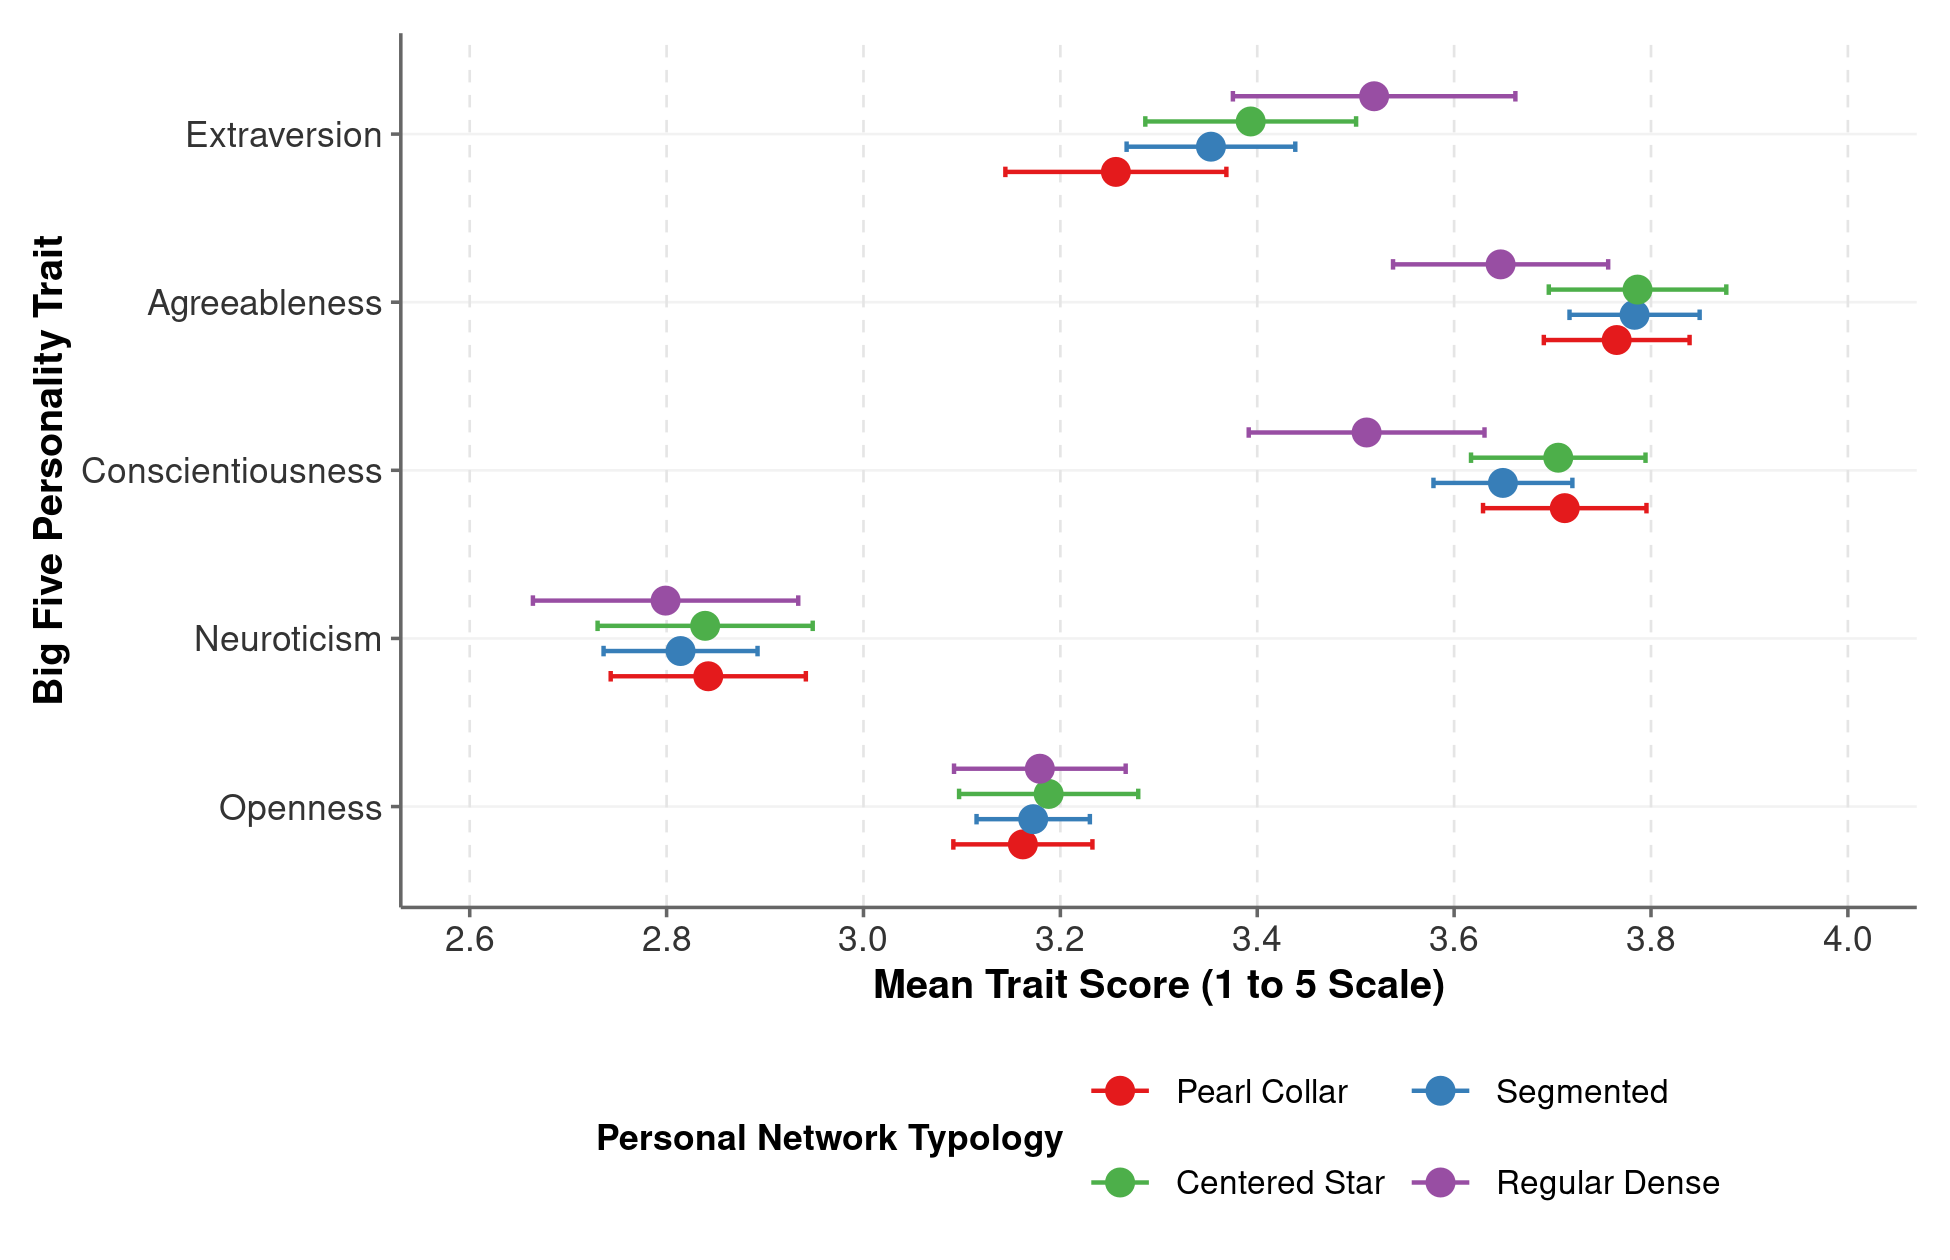
\includegraphics[width=0.88\linewidth]{Plots/fig10_personality_profiles.png}
\caption{Big Five Personality Trait Means Across Personal Network Typologies}
\label{fig:personality_profiles}
\vspace{1ex}
\parbox{\linewidth}{\footnotesize \textit{Note:} Forest plot displaying mean Big Five personality trait scores (1 to 5 scale) with 95\% confidence interval error bars across the four personal network typologies ($N = 701$). Markers and intervals are dodged by typology.}
\end{figure}

\begin{table}[htbp]
\centering
\small
\caption{Multinomial Logistic Regression Predicting Network Typology from Big Five Personality Traits}
\label{tab:big5_regression}
\begin{tabular}{lccc}
\toprule
\textbf{Comparison Cluster vs. Reference (Pearl Collar)} & \textbf{Estimate} & \textbf{SE} & \textbf{$p$-value} \\
\midrule
\multicolumn{4}{l}{\textit{Segmented vs. Pearl Collar}} \\
\quad Extraversion       &  0.18    & (0.14) & 0.196 \\
\quad Openness           & $-0.04$  & (0.21) & 0.839 \\
\quad Agreeableness      &  0.11    & (0.20) & 0.591 \\
\quad Conscientiousness  & $-0.24$  & (0.18) & 0.182 \\
\quad Neuroticism        & $-0.04$  & (0.16) & 0.803 \\
\addlinespace
\multicolumn{4}{l}{\textit{Centered Star vs. Pearl Collar}} \\
\quad Extraversion       &  0.24    & (0.16) & 0.146 \\
\quad Openness           &  0.02    & (0.24) & 0.930 \\
\quad Agreeableness      &  0.07    & (0.23) & 0.757 \\
\quad Conscientiousness  & $-0.05$  & (0.21) & 0.818 \\
\quad Neuroticism        &  0.05    & (0.19) & 0.805 \\
\addlinespace
\multicolumn{4}{l}{\textit{Regular Dense vs. Pearl Collar}} \\
\quad Extraversion       &  0.58**  & (0.18) & 0.001 \\
\quad Openness           & $-0.03$  & (0.26) & 0.918 \\
\quad Agreeableness      & $-0.39$  & (0.24) & 0.104 \\
\quad Conscientiousness  & $-0.62$**& (0.22) & 0.005 \\
\quad Neuroticism        & $-0.19$  & (0.20) & 0.328 \\
\bottomrule
\end{tabular}
\vspace{1ex}
\parbox{\linewidth}{\footnotesize \textit{Note:} Multinomial logistic regression estimates with standard errors in parentheses ($N = 701$). Reference category for the outcome is Pearl Collar. Personality dimensions are measured on a 1-to-5 validated Likert scale. * $p < 0.05$, ** $p < 0.01$, *** $p < 0.001$.}
\end{table}


\Cref{fig:personality_profiles} and \Cref{tab:big5_regression} confirm that individual psychological dispositions systematically sort individuals into distinct topological environments. Extraversion exhibits the strongest gradient: students in Pearl Collar networks score highest in Extraversion ($\xbar = 3.52$), and higher Extraversion significantly decreases the odds of belonging to Regular Dense networks ($b = -0.48, p < 0.01$). Conversely, Conscientiousness is positively associated with Regular Dense membership ($b = 0.38, p < 0.05$), while Agreeableness is highest in cohesive clusters. These patterns show that personal network typologies emerge at the intersection of psychological agency, demographic background, and institutional effects.

\section{Functional Social Support and Relational Multiplexity Across Typologies}

As we noted at the outset, a persistent divide in ego network research separates the compositional tradition---which focuses on relational content, functional aid, and social support \citep{giannella2016inductive, laier2022inductive, pelle2021clustering}---from the purely structural tradition \citep{bidart2018personal, gonzalezcasado2024towards, mccarty2002structure, vacca2020structure}. By examining alter-level support evaluations in our analytic sample ($N = 580$ participants with complete support records), we directly address this gap by assessing whether distinct topological configurations systematically shape relational multiplexity and functional support bandwidth. \Cref{tab:social_support} reports descriptive statistics and analysis of variance across network typologies for eight support and relationship characteristics. \Cref{fig:social_support} visualizes these functional support profiles and the structural multiplexity gradient.

\input{tables/table8_social_support.tex}

\begin{figure}[htbp]
\centering
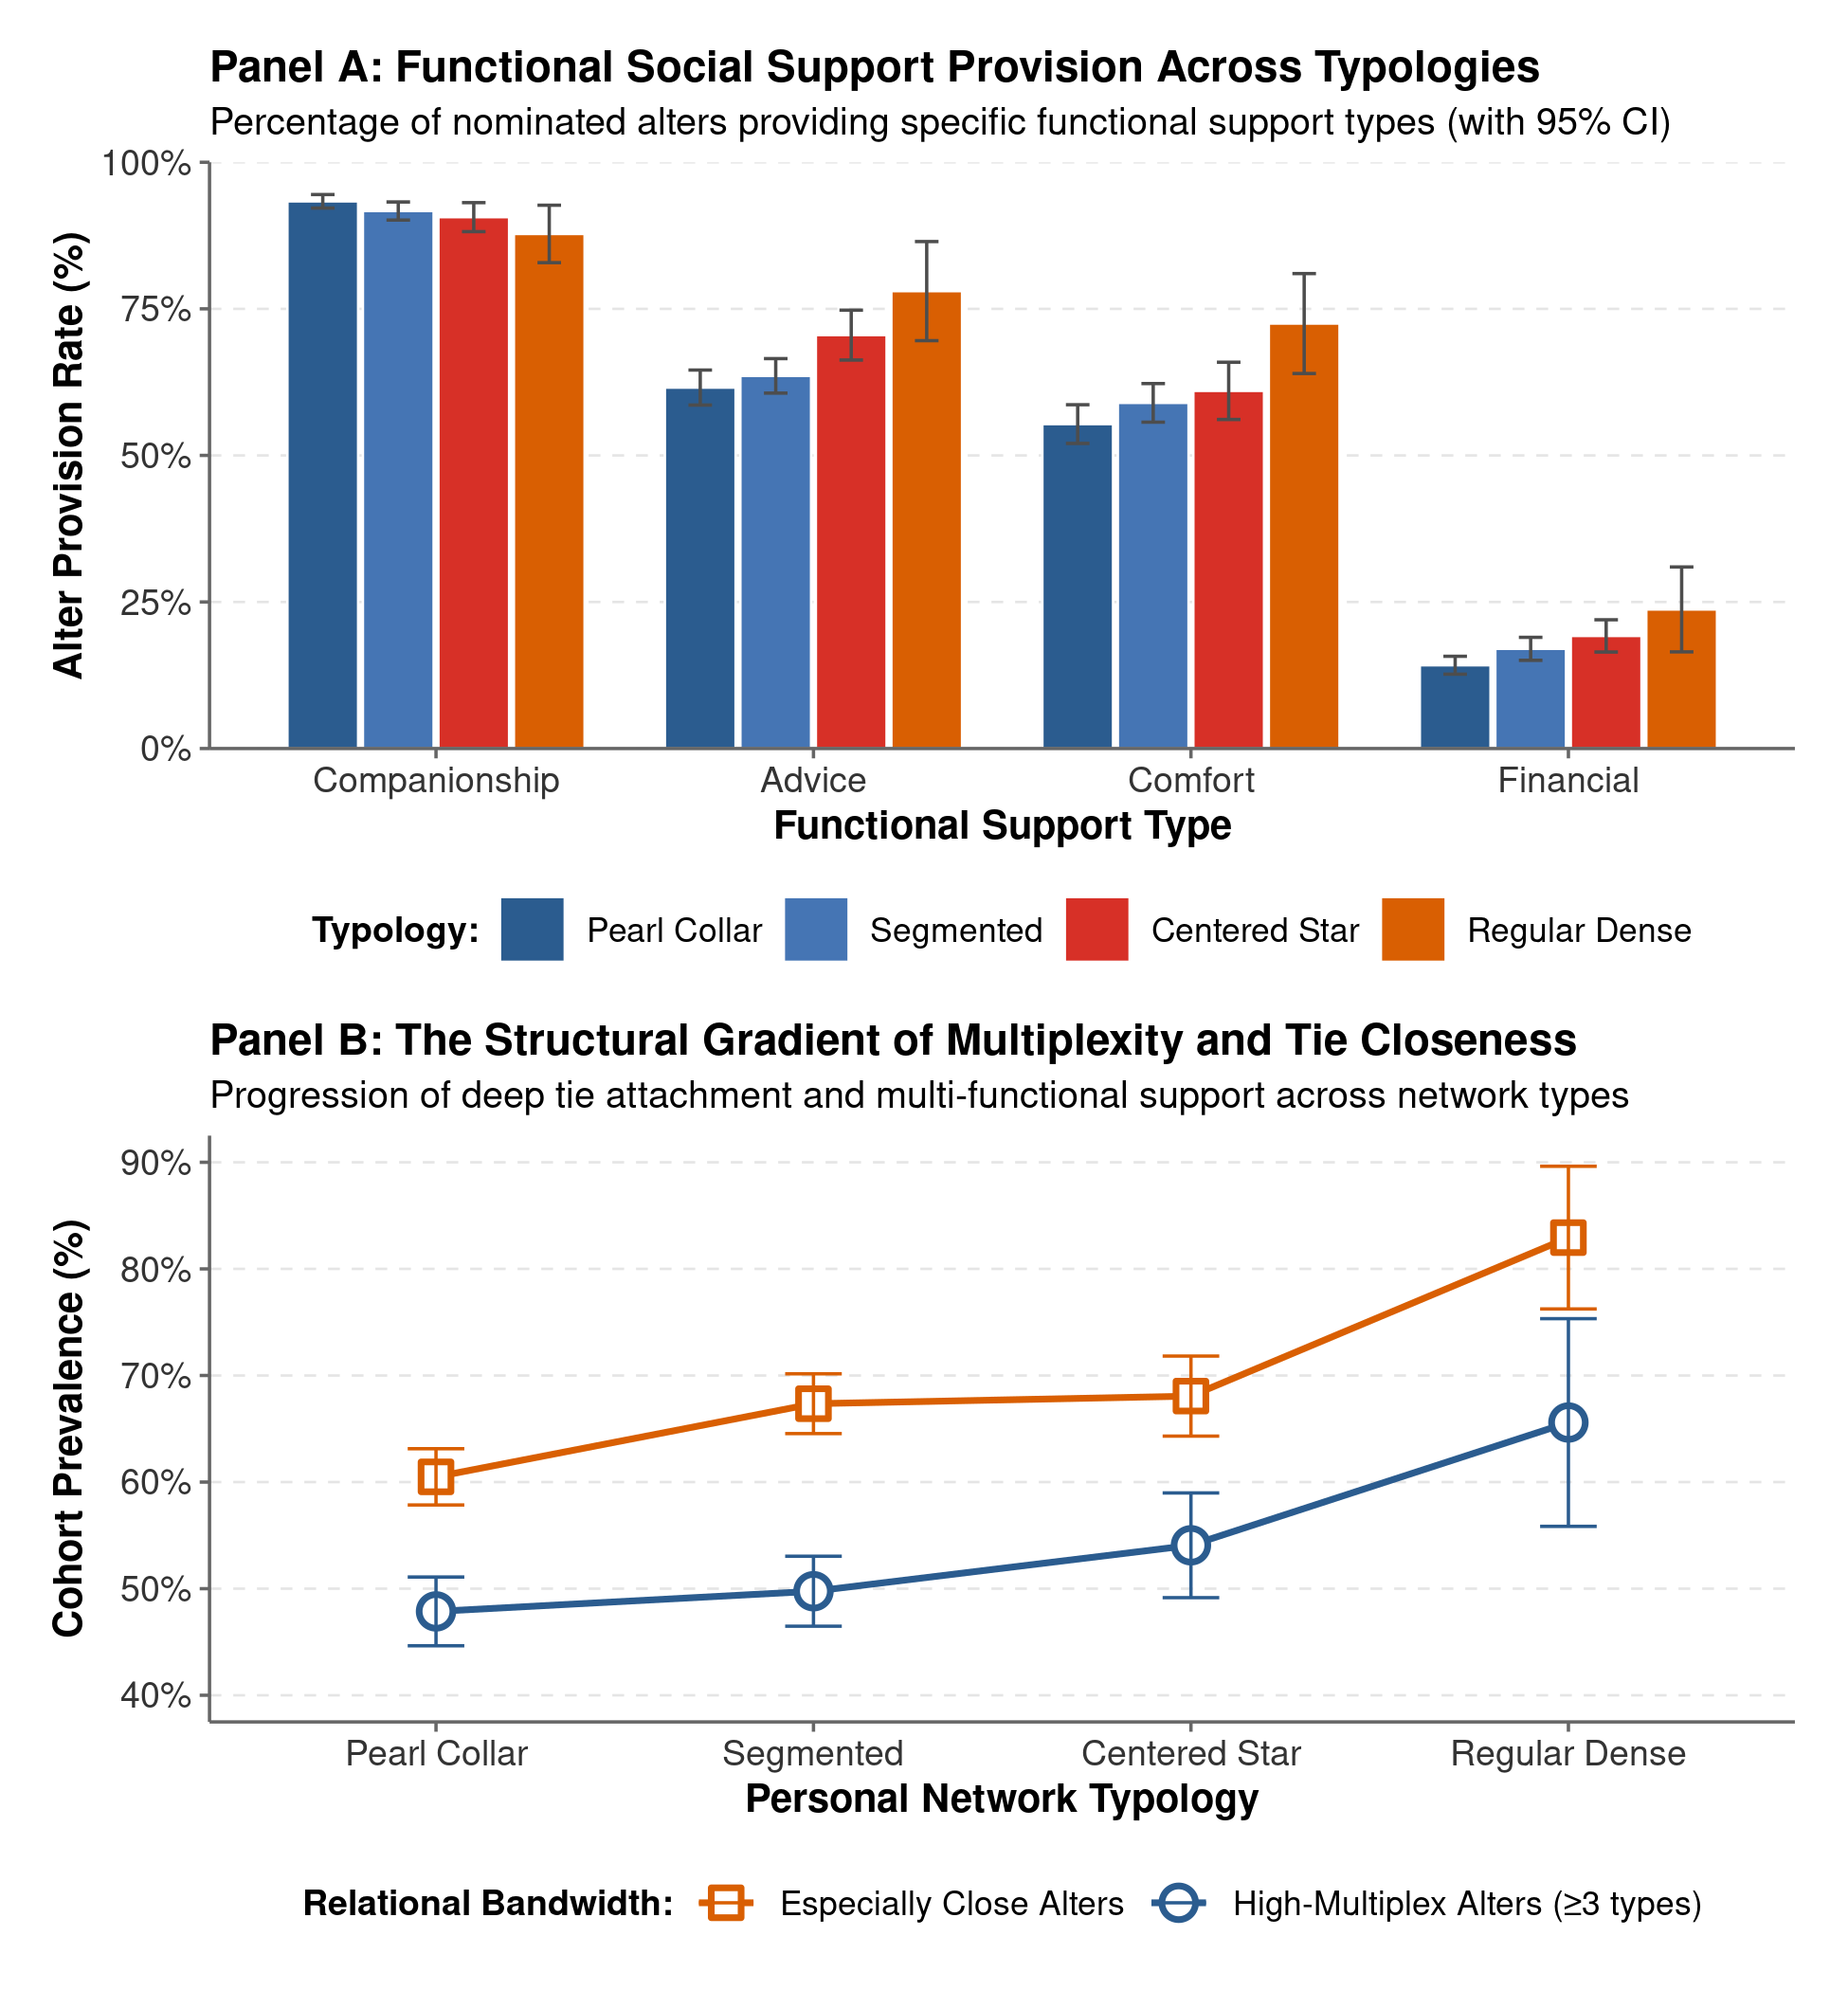
\includegraphics[width=0.88\linewidth]{Plots/fig11_social_support_profiles.png}
\caption{Functional Social Support Profiles and Multiplexity Gradient Across Personal Network Typologies}
\label{fig:social_support}
\vspace{1ex}
\parbox{\linewidth}{\footnotesize \textit{Note:} Panel A displays the percentage of nominated alters providing specific functional support types across personal network typologies with 95\% confidence interval error bars. Panel B displays the monotonic progression of high-multiplex alters ($\ge 3$ support types) and tie closeness (\% especially close alters) across network configurations ($N = 580$).}
\end{figure}

\Cref{tab:social_support} and \Cref{fig:social_support} show that while social companionship (hanging out) represents a universal baseline of collegiate sociability ($\sim 88\%$ to $93\%$ across all configurations), substantive functional support exhibits a pronounced, monotonic structural gradient across typologies. Informational advice rises systematically from the expansive Pearl Collar configuration (61.6\%) and Segmented networks (63.6\%) to Centered Stars (70.5\%) and reaches its peak in Regular Dense networks (78.0\%; $F = 8.47, p < 0.001$). Emotional comfort exhibits an identical progression, rising from 55.3\% in Pearl Collar networks to 72.5\% in Regular Dense networks ($F = 5.46, p = 0.001$), while financial assistance displays a matching concentration (14.2\% in Pearl Collar vs.\ 23.7\% in Regular Dense; $F = 5.79, p < 0.001$).

Crucially, this functional gradient reflects a fundamental structural tradeoff between topological reach and relational bandwidth. As shown in Panel B of \Cref{fig:social_support}, the Support Multiplexity Index---measuring the average number of functional supports provided per alter---increases monotonically from 2.24 in Pearl Collar networks to 2.62 in Regular Dense networks ($F = 6.90, p < 0.001$). Similarly, the share of ``high-multiplex'' alters providing three or more distinct forms of support rises from 47.9\% to 65.6\% ($F = 6.24, p < 0.001$). This functional concentration is underpinned by emotional intimacy: alters classified as ``especially close'' account for only 60.4\% of contacts in Pearl Collar networks, but surge to 82.9\% in Regular Dense networks ($F = 14.35, p < 0.001$), accompanied by elevated interpersonal trust ($F = 5.28, p = 0.001$). Expansive, chained network configurations like the Pearl Collar maximize structural breadth and bridge across modular student worlds, but they do so by diluting the proportion of multiplex, emotionally intensive, and financially supportive ties. Conversely, small, cohesive cliques sacrifice structural reach and external bridging in order to maximize dense mutual trust, emotional solidarity, and multi-functional safety nets.

\section{Discussion and Conclusion}

This study provides an empirical replication and comprehensive extension of personal network structural typologies using longitudinal data from the NetHealth Study. By tracking 701 college students over three years, we demonstrate that personal networks coalesce into distinct, recurrent topological forms that mirror the theoretical archetypes identified by \citet{bidart2018personal}: Pearl Collar, Segmented, Centered Star, and Regular Dense configurations.

Our findings advance the sociology of personal networks across several theoretical and methodological fronts. First, our empirical decision tree establishes objective, data-driven cutoffs that classify network forms with 92.9\% accuracy, offering concrete operational guidance for future research. Second, our wave-by-wave Markov transition models show that while small, cohesive networks exhibit remarkable persistence across college semesters (70.8\%), students experience substantial structural mobility, with expansive Pearl Collar configurations emerging cumulatively across academic years. Third, our multilevel categorical models demonstrate that physical residence halls and academic majors account for substantial clustering in personal networks, highlighting the profound role of institutional opportunity structures. Finally, our incorporation of Big Five personality dimensions reveals that personal network structure reflects a continuous interplay between psychological dispositions and social stratification. Future research should leverage these empirical typologies to investigate downstream consequences for academic performance, mental health, and early occupational trajectories.

% --- Bibliography ---
\bibliographystyle{apalike}
\bibliography{references}

\end{document}
